% GhostVault: Encrypted File Storage Across Private GitHub Repositories
% System Design and Implementation Report
%
% Build with XeLaTeX (two runs, for the cross-references):
%     latexmk -xelatex ghostvault-report.tex        or        make
% Fonts: TeX Gyre Termes and TeX Gyre Heros (TeX Live), Liberation Mono.
% Figures are TikZ/pgfplots sources in figures/; the data behind the charts is in data/.

\documentclass[10pt,twocolumn,letterpaper]{article}
\usepackage[letterpaper,top=0.75in,bottom=0.9in,left=0.625in,right=0.625in,columnsep=0.25in]{geometry}

\usepackage{amsmath}
\usepackage{mathptmx}
\usepackage{fontspec}
\setmainfont{TeX Gyre Termes}
\setsansfont{TeX Gyre Heros}[Scale=MatchLowercase]
\setmonofont{Liberation Mono}[Scale=0.84]
\usepackage{microtype}
\usepackage{xcolor,graphicx}
\usepackage{tikz}
\usetikzlibrary{arrows.meta,positioning,fit,calc,backgrounds,shapes.geometric}
\usepackage{pgfplots}
\pgfplotsset{compat=1.18}
\usepackage{array,booktabs,tabularx,multirow}
\usepackage{titlesec}
\usepackage{caption}
\usepackage{listings}
\usepackage{enumitem}
\usepackage{stfloats}
\usepackage{xurl}
\usepackage[hidelinks,pdfusetitle]{hyperref}
\hypersetup{
  pdftitle={GhostVault: Encrypted File Storage Across Private GitHub Repositories},
  pdfsubject={System Design and Implementation Report, GhostVault 1.0.0},
  pdfkeywords={encrypted storage, authenticated encryption, AES-GCM, GitHub, Git object store,
               crash consistency, journaling, desktop application},
}

% ---- headings in the style of IEEE transactions ------------------------------------------------
\renewcommand{\thesection}{\Roman{section}}
\renewcommand{\thesubsection}{\thesection\mbox{-}\Alph{subsection}}
\titleformat{\section}{\normalsize\scshape\centering}{\thesection.}{0.5em}{}
\titlespacing*{\section}{0pt}{1.7ex plus .5ex minus .2ex}{0.8ex plus .2ex}
\titleformat{\subsection}{\normalsize\itshape}{\Alph{subsection}.}{0.5em}{}
\titlespacing*{\subsection}{0pt}{1.3ex plus .4ex minus .2ex}{0.4ex plus .1ex}

% ---- captions: TABLE I above in small capitals, Fig. 1 below ----------------------------------
\renewcommand{\thetable}{\Roman{table}}
\DeclareCaptionLabelFormat{upper}{\MakeUppercase{#1}~#2}
\captionsetup[table]{labelformat=upper, labelsep=newline, font={footnotesize,sc}, justification=centering,
                     skip=3pt}
\captionsetup[figure]{name=Fig., labelsep=period, font=footnotesize, justification=justified,
                      singlelinecheck=true, skip=4pt}
\captionsetup[lstlisting]{labelsep=period, font=footnotesize, justification=justified,
                          singlelinecheck=false, skip=3pt}

% ---- listings ----------------------------------------------------------------------------------------
\lstset{
  basicstyle=\ttfamily\footnotesize, columns=fullflexible, keepspaces=true,
  backgroundcolor=\color{black!4}, frame=single, rulecolor=\color{black!22}, framesep=3pt,
  xleftmargin=3.5pt, xrightmargin=3.5pt, aboveskip=6pt, belowskip=4pt,
  showstringspaces=false, upquote=true, breaklines=true, breakindent=1.5em,
  commentstyle=\color{black!55}, numbers=none, float=!htb,
}
\lstdefinelanguage{gvjson}{morestring=[b]", morecomment=[l]{//}}

% ---- floats, lists, small helpers ------------------------------------------------------------------
\renewcommand{\topfraction}{0.92}
\renewcommand{\dbltopfraction}{0.92}
\renewcommand{\bottomfraction}{0.6}
\renewcommand{\textfraction}{0.06}
\renewcommand{\floatpagefraction}{0.82}
\renewcommand{\dblfloatpagefraction}{0.82}
\setcounter{topnumber}{3}
\setcounter{dbltopnumber}{2}
\setlength{\textfloatsep}{10pt plus 2pt minus 3pt}
\setlength{\dbltextfloatsep}{12pt plus 2pt minus 3pt}
\setlength{\floatsep}{9pt plus 2pt minus 2pt}
\setlist{nosep, leftmargin=1.2em}
\setlist[enumerate]{leftmargin=1.5em}
\newcolumntype{L}[1]{>{\raggedright\arraybackslash}p{#1}}
\newcolumntype{Y}{>{\raggedright\arraybackslash}X}
\newcommand{\code}[1]{\texttt{#1}}
\newcommand{\state}[1]{\texttt{#1}}
\newcommand{\figref}[1]{Fig.~\ref{#1}}
\newcommand{\tabref}[1]{Table~\ref{#1}}
\newcommand{\secref}[1]{Section~\ref{#1}}
\newcommand{\lstref}[1]{Listing~\ref{#1}}
\newcommand{\KiB}{\,KiB}
\newcommand{\MiB}{\,MiB}
\newcommand{\GiB}{\,GiB}
\renewcommand{\arraystretch}{1.12}

\begin{document}
\fussy
\setlength{\emergencystretch}{1.2em}
\raggedbottom

\twocolumn[{%
\begin{center}
  {\fontsize{23}{27}\selectfont GhostVault: Encrypted File Storage Across\\[2pt]
   Private GitHub Repositories\par}
  \vspace{7pt}
  {\large\itshape System Design and Implementation Report\par}
  \vspace{4pt}
  {\small GhostVault 1.0.0 \quad\textperiodcentered\quad October 2026\par}
\end{center}
\vspace{12pt}
}]

\noindent{\small\bfseries\textit{Abstract}---GhostVault is a desktop application that moves files
off a computer into private GitHub repositories that the user owns, and brings them back on
request. A file is split into 512\,KiB chunks, and each chunk is encrypted on the computer with
AES-256-GCM under a random key used for that file alone; its associated data binds the chunk to
the file, its position, the number of chunks, the file's exact size and whether it is padded. The
chunks are stored as Git blobs, with one commit per repository. The original is deleted only after
each repository's branch has been read back and lists every chunk under the content id computed
before the upload, a sample of chunks has been downloaded and compared, and the file on disk has
been shown, once more, to be the one that was uploaded. Every step that changes something outside
the application is preceded by a durable journal entry, so an interruption at any point is
finished or undone at the next start. Encrypted recovery files and an optional encrypted backup
kept in the repositories protect against losing the computer. This report describes the system:
its parts and formats, its operations and their failure handling, and where its protection ends,
separating what the cryptography guarantees from what depends on GitHub's access control and on
GitHub keeping the data. It also reports how the system was checked: an automated suite of 663
tests, a randomised run of 3\,200 operations with 1\,273 simulated crashes and 7\,736 injected
network faults in which no file was lost, and measurements of its own costs.\par}

\vspace{6pt}
\noindent{\small\bfseries\textit{Index Terms}---Encrypted storage, authenticated encryption,
AES-GCM, Git object storage, GitHub, crash consistency, write-ahead journaling, desktop
application.\par}
\vspace{4pt}

\section{Introduction}\label{sec:intro}

\subsection{The problem}
Many files must be kept but are rarely opened: finished projects, scans, archives, old
photographs. Keeping them on the computer costs space; moving them to a storage service hands
them to a provider that can read them, or that holds the keys that would let it. Many people who
write software already have something else: private GitHub repositories, reached through a
well-documented HTTPS interface, with an access-controlled place to put data.

Two facts stand in the way of simply putting files there. A private repository is private only
by GitHub's access control: GitHub, every collaborator, and anyone holding a token with access
can read every byte of it, and so can everyone if the repository is ever made public. And GitHub
is explicit that ``Git is not designed to serve as a backup tool''~\cite{gh-large}; a repository
can be deleted, an account suspended, a token revoked.

\subsection{The idea}
GhostVault treats the repositories as an untrusted store of opaque objects. A file is
\emph{ghosted}: it is encrypted on the computer, uploaded in chunks, checked on GitHub, and then
removed from the computer. What remains locally is a \emph{ghost}: a small record that holds the
file's key and the location of every chunk, shown as a card in GhostVault's window.
\emph{Restoring} a ghost downloads and checks its chunks, writes the file into a folder the user
chooses, and then removes its copy from GitHub. Everything GitHub receives about a file is
encrypted: it never sees the file's key, its name or its content.

The consequence that shapes the whole design is that GhostVault deletes the user's files on
purpose. Encryption is the easier part; the harder part is deciding, after crashes, network
failures, misleading replies and other programs touching the same files, when a deletion is
allowed. The original is deleted only once its encrypted copy has been shown to be on GitHub, and
the remote copy only once the restored file is safely on disk. Most of this report is about how
those two decisions are made and recorded.

\subsection{What this report covers}
This is a systems report about GhostVault 1.0.0. It describes what the system is made of, the
formats it writes, the rules its operations follow and why, and how it was checked. Every
statement about behaviour was checked against the source code; every number comes from a
measurement whose method is given, run on one stated machine; and what has not been verified is
listed in \secref{sec:status}. The report aims to be as precise about what GhostVault does not do
as about what it does.

\secref{sec:overview} gives an overview and \secref{sec:principles} the principles behind the
design. \secref{sec:threats} sets out the threat model and the boundaries of the protection.
Sections~\ref{sec:crypto} to \ref{sec:recovery} describe the cryptography, the local state and
its journal, ghosting, restoring, the use of GitHub, and recovery.
Sections~\ref{sec:app} and~\ref{sec:impl} cover the desktop application, its standalone builds and
the implementation. Sections~\ref{sec:verification} and~\ref{sec:performance} report verification
and performance, and \secref{sec:limitations} the limitations.

\section{System Overview}\label{sec:overview}

\begin{figure*}[t]
\centering
% Fig.: the components of GhostVault and what they talk to.
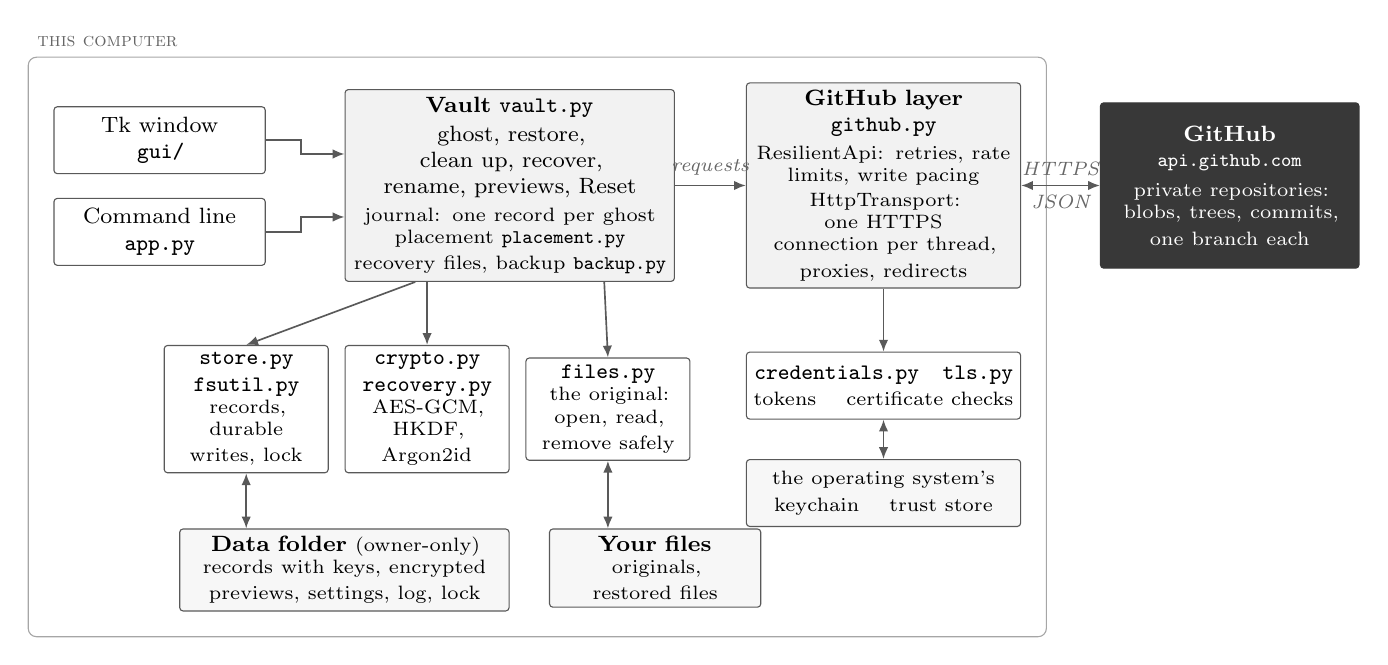
\begin{tikzpicture}[
  font=\footnotesize,
  node distance=4mm,
  box/.style={draw=black!65, fill=white, rounded corners=1.2pt, align=center, inner sep=2.6pt,
              minimum height=8.5mm, text width=#1},
  box/.default=27mm,
  core/.style={box=#1, fill=black!5},
  dark/.style={box=#1, fill=black!78, draw=black!78, text=white},
  region/.style={draw=black!35, rounded corners=3pt, inner sep=3.2mm},
  title/.style={font=\scriptsize\scshape, text=black!60, anchor=south west},
  arr/.style={-{Latex[length=1.5mm,width=1.2mm]}, draw=black!65, semithick},
  both/.style={{Latex[length=1.5mm,width=1.2mm]}-{Latex[length=1.5mm,width=1.2mm]}, draw=black!65, semithick},
  note/.style={font=\scriptsize\itshape, text=black!60, align=center},
]
% --- the user's side -------------------------------------------------------------------------
\node[box=25mm] (gui) {Tk window\\\texttt{gui/}};
\node[box=25mm, below=3mm of gui] (cli) {Command line\\\texttt{app.py}};

% --- the core --------------------------------------------------------------------------------
\node[core=40mm, right=10mm of gui, yshift=-5.75mm, minimum height=21mm] (vault)
  {\textbf{Vault} \texttt{vault.py}\\[1pt]
   ghost, restore, clean up, recover,\\ rename, previews, Reset\\[2pt]
   \scriptsize journal: one record per ghost\\
   \scriptsize placement \texttt{placement.py}\\
   \scriptsize recovery files, backup \texttt{backup.py}};

\node[box=19mm, below=8mm of vault.south west, anchor=north west] (crypto)
  {\texttt{crypto.py}\\\texttt{recovery.py}\\\scriptsize AES-GCM, HKDF,\\\scriptsize Argon2id};
\node[box=19mm, right=2mm of crypto] (files)
  {\texttt{files.py}\\\scriptsize the original:\\\scriptsize open, read,\\\scriptsize remove safely};
\node[box=19mm, left=2mm of crypto] (store)
  {\texttt{store.py}\\\texttt{fsutil.py}\\\scriptsize records, durable\\\scriptsize writes, lock};

% --- GitHub layer ----------------------------------------------------------------------------
\node[core=33mm, right=9mm of vault, minimum height=21mm] (gh)
  {\textbf{GitHub layer} \texttt{github.py}\\[2pt]
   \scriptsize ResilientApi: retries, rate\\\scriptsize limits, write pacing\\[1pt]
   \scriptsize HttpTransport: one HTTPS\\\scriptsize connection per thread,\\\scriptsize proxies, redirects};
\node[box=33mm, below=8mm of gh] (keys)
  {\texttt{credentials.py}\quad \texttt{tls.py}\\\scriptsize tokens \quad certificate checks};

% --- outside GhostVault ----------------------------------------------------------------------
\node[dark=31mm, right=10mm of gh, minimum height=21mm] (github)
  {\textbf{GitHub}\\[1pt]\scriptsize \texttt{api.github.com}\\[3pt]
   \scriptsize private repositories:\\\scriptsize blobs, trees, commits,\\\scriptsize one branch each};
\node[box=33mm, below=5mm of keys, fill=black!3] (os)
  {\scriptsize the operating system's\\\scriptsize keychain \quad trust store};

\node[box=40mm, below=7mm of crypto.south, anchor=north, xshift=-10.5mm, fill=black!3] (folder)
  {\textbf{Data folder} \scriptsize (owner-only)\\\scriptsize records with keys, encrypted\\\scriptsize previews, settings, log, lock};
\node[box=25mm, anchor=north, fill=black!3] (yours) at ([xshift=6mm]files.south |- folder.north)
  {\textbf{Your files}\\\scriptsize originals,\\\scriptsize restored files};

% --- arrows ----------------------------------------------------------------------------------
\draw[arr] (gui.east) -- ++(4.5mm,0) |- ([yshift=4mm]vault.west);
\draw[arr] (cli.east) -- ++(4.5mm,0) |- ([yshift=-4mm]vault.west);
\draw[arr] (vault.east) -- node[above, note] {requests} (gh.west);
\draw[both] (gh.east) -- node[above, note] {HTTPS} node[below, note] {JSON} (github.west);
\draw[arr] (gh.south) -- (keys.north);
\draw[both] (keys.south) -- (os.north);
\draw[arr] (vault.south -| crypto.north) -- (crypto.north);
\draw[arr] ([xshift=-12mm]vault.south) -- (store.north);
\draw[arr] ([xshift=12mm]vault.south) -- (files.north);
\draw[both] (store.south) -- (store.south |- folder.north);
\draw[both] (files.south) -- (files.south |- yours.north);

% --- regions ---------------------------------------------------------------------------------
\begin{scope}[on background layer]
  \node[region, fit=(gui)(cli)(vault)(gh)(keys)(os)(store)(files)(folder)(yours)] (pc) {};
\end{scope}
\node[title] at (pc.north west) {this computer};
\end{tikzpicture}

\caption{The parts of GhostVault. Everything inside the frame runs on the user's computer;
GhostVault has no server of its own. The core (\code{Vault} and the modules below it) never imports
the user interface. Only the GitHub layer talks to the network, and only to \code{api.github.com}.}
\label{fig:architecture}
\end{figure*}

\subsection{The parts}
GhostVault has three parts, shown in \figref{fig:architecture}.

\emph{The application} is one Python package, \code{ghostvault}. A Tk window is the normal way to
use it; a command line offers recovery operations and a self-check. It runs from the Python
package or as a standalone application with its own Python inside (\secref{sec:builds}).

\emph{The data folder} is a per-user folder that only the user can read. It holds one record per
ghost, the settings, an encrypted cache of image previews and a log. Its location follows each
system's convention (\secref{sec:folder}).

\emph{The repositories} are one or more private GitHub repositories, each with a token that can
write to it. GhostVault reaches them through GitHub's REST API over HTTPS and stores its objects in
one folder of each, \code{ghostvault/}. It has no server, account or service of its own: if
GhostVault's authors disappeared, every ghost would remain restorable with the application, the
data folder and the repositories.

\subsection{What a ghost is}
A ghost is two things: its record in the data folder, and its chunks on GitHub. The record
(\lstref{lst:record}) holds the file's key; for every chunk, the repository it went to, its
random path, its nonce and the ids that identify its ciphertext; the original's name, location,
size, SHA-256, permissions and timestamps; and the journal state of the operation in progress.
The chunks are encrypted, by default padded to one size, and named at random.

The record is the only map from a ghost to its chunks and the only copy of its key. The gallery
in the window is simply the set of readable records; there is no separate index that could
disagree with them. Losing a record without a recovery bundle (\secref{sec:recovery}) loses the
ghost, whatever GitHub still holds.

\subsection{The life of a file}
\figref{fig:lifecycle} shows the two operations step by step. Ghosting plans the upload, records
the plan, uploads and commits the chunks, verifies them on GitHub, and only then removes the
original. Restoring records where the file will go, downloads and checks every chunk, writes and
publishes the file, and only then removes the chunks from GitHub. The grey tags are the journal
states written to disk before the step they precede; they are what start-up recovery reads after
an interruption (\secref{sec:journal}).

\begin{figure}[t]
\centering
% Fig.: the steps of ghosting and restoring, and the journal state written before each step.
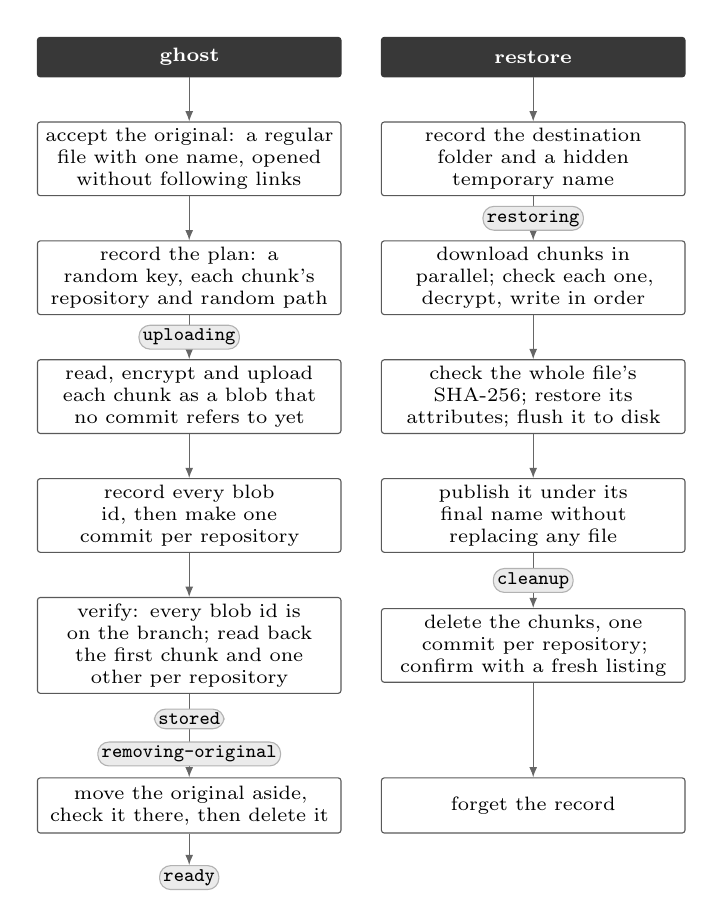
\begin{tikzpicture}[
  font=\scriptsize,
  stage/.style={draw=black!65, fill=white, rounded corners=1pt, align=center, text width=37mm,
               inner sep=2.2pt, minimum height=7mm,
               execute at begin node={\hyphenpenalty=10000\exhyphenpenalty=10000}},
  head/.style={stage, fill=black!78, draw=black!78, text=white, font=\scriptsize\bfseries, minimum height=5mm},
  arr/.style={-{Latex[length=1.3mm,width=1mm]}, draw=black!60},
  state/.style={fill=black!8, draw=black!30, rounded corners=4pt, inner sep=1.4pt, font=\scriptsize\ttfamily},
]
\matrix[row sep=5.6mm, column sep=5mm] (m) {
  \node[head] (g0) {ghost}; &
  \node[head] (r0) {restore}; \\
  \node[stage] (g1) {accept the original: a regular file with one name, opened without following links}; &
  \node[stage] (r1) {record the destination folder and a hidden temporary name}; \\
  \node[stage] (g2) {record the plan: a random key, each chunk's repository and random path}; &
  \node[stage] (r2) {download chunks in parallel; check each one, decrypt, write in order}; \\
  \node[stage] (g3) {read, encrypt and upload each chunk as a blob that no commit refers to yet}; &
  \node[stage] (r3) {check the whole file's SHA-256; restore its attributes; flush it to disk}; \\
  \node[stage] (g4) {record every blob id, then make one commit per repository}; &
  \node[stage] (r4) {publish it under its final name without replacing any file}; \\
  \node[stage] (g5) {verify: every blob id is on the branch; read back the first chunk and one other per repository}; &
  \node[stage] (r5) {delete the chunks, one commit per repository; confirm with a fresh listing}; \\[5mm]
  \node[stage] (g6) {move the original aside, check it there, then delete it}; &
  \node[stage] (r6) {forget the record}; \\
};
\foreach \a/\b in {g0/g1, g1/g2, g2/g3, g3/g4, g4/g5, g5/g6, r0/r1, r1/r2, r2/r3, r3/r4, r4/r5, r5/r6}
  \draw[arr] (\a) -- (\b);
% journal states, written durably before the step below them (drawn on the arrow)
\node[state] at ($(g2.south)!0.5!(g3.north)$) {uploading};
\node[state] at ($(g5.south)!0.3!(g6.north)$) {stored};
\node[state] at ($(g5.south)!0.72!(g6.north)$) {removing-original};
\node[state, below=4mm of g6] (ready) {ready};
\draw[arr] (g6) -- (ready);
\node[state] at ($(r1.south)!0.5!(r2.north)$) {restoring};
\node[state] at ($(r4.south)!0.5!(r5.north)$) {cleanup};
\end{tikzpicture}

\caption{Ghosting and restoring a file. Each grey tag is the journal state written durably before
the step below it. Nothing is deleted on either side until the other copy has been checked.}
\label{fig:lifecycle}
\end{figure}

\section{Design Principles}\label{sec:principles}

Eight rules shape the design; the rest of the report shows where each applies.

\emph{Delete only what has a checked second copy.} The original is deleted only after GitHub's
branch has been read back and shows every chunk under the id computed locally from its
ciphertext, a sample has been downloaded and compared, and the file is still the one that was
read. Remote chunks are deleted only after the restored file has been written, checked, flushed
to disk and given its final name.

\emph{Record the intent before acting.} Every step that changes something outside the data folder
is preceded by a durable record of what is about to happen. The record names everything the step
could create (chunk paths are chosen at random and recorded before the first upload), so nothing
can appear on GitHub that GhostVault could not find and remove.

\emph{A reply is not proof.} A reply can be lost, can come from a lagging replica, or can report
success for a change that did not take effect. Wherever an outcome matters, GhostVault reads the
branch again and acts on what it shows.

\emph{GitHub stores; it is not trusted with secrets or integrity.} Only ciphertext under keys
GitHub never sees is uploaded, and every byte that comes back is checked against its content id,
its SHA-256 and its authentication tag before it is used.

\emph{One random key per file.} File keys are random, never derived from a password, so a weak
passphrase can weaken only the recovery bundle it protects, and a key that leaks exposes one file.

\emph{Validate before acting.} A record is validated every time it is read. Every value used to
build a request, choose a path or delete something must have the only form GhostVault itself
creates, so a damaged or edited record cannot direct a deletion at anything that is not
GhostVault's own.

\emph{When in doubt, keep the data.} An unreadable record is reported and never overwritten; a
damaged settings file is moved aside, never deleted; an original that changed is kept; a backup
that fails never fails the operation that triggered it.

\emph{Say what is true.} Status shown to the user reflects what was verified. A ghost counts as
protected by the repository backup only once that version has been read back from GitHub, and a
file whose original could not be deleted is reported as kept, with the reason.

\section{Threat Model and Security Boundaries}\label{sec:threats}

\subsection{Three different kinds of protection}
It is easy to read ``encrypted files in private repositories'' as one guarantee. It is three, with
different owners, and GhostVault provides only the first.

\emph{The content of a file is protected by cryptography.} Its confidentiality and integrity hold
against anyone who can read or change the repositories, GitHub included, as long as the keys stay
secret and AES-GCM is secure. Nothing about this depends on the repositories being private.

\emph{Who can read the repositories is decided by GitHub's access control.} ``Private'' is a
GitHub setting, not encryption. GhostVault refuses a repository that is public, archived or not
writable with the given token when it is added (\secref{sec:gh-checks}), but afterwards GitHub
alone decides who can read it: collaborators, holders of any token with access, GitHub itself,
and everyone if the repository is ever made public. Because of the encryption, what such readers
gain is limited to the metadata in \tabref{tab:learn}; but they do gain that.

\emph{Whether the data is still there is decided by GitHub.} Each chunk is stored exactly once.
If a repository is deleted, an account suspended, a token's access withdrawn for good or the data
lost, every ghost with a chunk there is lost; GitHub's acceptable use policies reserve the right
to ``suspend your Account, throttle your file hosting, or otherwise limit your activity'' when
bandwidth use is ``significantly excessive''~\cite{gh-aup}. GhostVault detects missing or damaged
data and refuses to restore it wrongly; it cannot bring it back. And once a file is ghosted, the
ghost is its only copy unless the user keeps others.

\begin{table*}[t]
\caption{Who the design considers, what they can do, and what stops them}\label{tab:parties}
\centering\footnotesize
\begin{tabularx}{\textwidth}{@{}L{36mm}L{48mm}Y@{}}
\toprule
\textbf{Party or event} & \textbf{Can} & \textbf{What GhostVault does about it} \\
\midrule
GitHub, or anyone who can read the repositories & read every blob, tree and commit, with their
times and history & only ciphertext under keys they never see; random paths; neutral commit
messages; padding hides exact sizes. They learn what \tabref{tab:learn} lists. \\ \addlinespace[1.6pt]
Someone on the network & read or change traffic & TLS, with GitHub's certificate verified against
the operating system's trust store. \\ \addlinespace[1.6pt]
Someone who changes the data on GitHub & change, swap, truncate or delete chunks & detected: every
chunk is checked against its content id, its SHA-256 and its GCM tag, whose associated data binds
file, position, count, size and padding. A restore fails without writing anything under the file's
name. Deleted data cannot be brought back. \\ \addlinespace[1.6pt]
Crashes, power loss, a full disk, network failures & interrupt any operation at any point & every
step that changes something outside the data folder is journaled first; the next start finishes or
undoes it (\secref{sec:journal}). \\ \addlinespace[1.6pt]
Another program working on the same files & replace, edit or rename the original or the restored
file's name while GhostVault works & the original is moved to a hidden name and checked there before
it is deleted; a restored file is published without replacing anything (Sections~\ref{sec:remove}
and~\ref{sec:publish}). \\ \addlinespace[1.6pt]
Another account on the computer, a stolen disk, a copy of the data folder & read what file
permissions let them read & partly: the data folder is readable by its owner only, but the keys
in it are not encrypted (\secref{sec:keys}); disk encryption and protected backups of the folder
are the user's part. \\ \addlinespace[1.6pt]
Malware running as the user & everything the user can do & not covered: it can read the data
folder and the keychain and watch what is opened. \\ \addlinespace[1.6pt]
A compromised dependency, build tool or release & run code inside GhostVault & partly:
dependencies are audited in CI, build tools are pinned, releases carry SHA-256 checksums, and builds
are signed when a certificate is configured (\secref{sec:builds}). \\
\bottomrule
\end{tabularx}
\end{table*}

\subsection{Parties and events}
\tabref{tab:parties} lists who the design considers and what stops each of them. GhostVault
trusts the operating system, the user's account, the Python runtime, the \code{cryptography}
library and the OpenSSL inside it, and the operating system's certificate store for TLS. It does
not trust GitHub's replies, the state of a file between two system calls, or its own state files
after a crash; each is checked before anything depends on it.

\subsection{What GitHub learns}\label{sec:learn}
\tabref{tab:learn} lists what anyone who can read the repositories learns, and what stays hidden.
Commit messages are always \code{Update}, and paths are random, so neither the tree nor the history
names a file. A network observer sees only that the computer talks to \code{api.github.com}, how
much and when.

\begin{table}[t]
\caption{What readers of the repositories learn}\label{tab:learn}
\centering\footnotesize
\begin{tabular}{@{}L{40mm}L{40mm}@{}}
\toprule
\textbf{They learn} & \textbf{They do not learn} \\
\midrule
that the account stores GhostVault-shaped encrypted data, and how much & file names, types or
content \\ \addlinespace[1.6pt]
each ghost's chunk count, so its size to within 512\,KiB with padding (the default), or exactly
without & the exact size, when padding is on \\ \addlinespace[1.6pt]
when each ghost was uploaded and removed, where, and which chunks were committed together &
original paths, timestamps, or hashes of the plaintext \\ \addlinespace[1.6pt]
whether a ghost has a preview (all previews have one size) & what a preview shows, or its
dimensions \\ \addlinespace[1.6pt]
the account's addresses and active times & keys, nonces or tokens \\
\bottomrule
\end{tabular}
\end{table}

\section{Cryptographic Design}\label{sec:crypto}

GhostVault defines no cryptographic algorithm of its own. It uses AES-256-GCM~\cite{nist-gcm},
HKDF-SHA256~\cite{rfc5869}, Argon2id~\cite{rfc9106} (or scrypt~\cite{rfc7914} where the
\code{cryptography} build has no Argon2id) and HMAC-SHA256~\cite{rfc2104}, all from the
\code{cryptography} library~\cite{pyca}, and SHA-256 for content checks.

\begin{figure*}[t]
\centering
% Fig.: the keys, what each is made from, and what each protects.
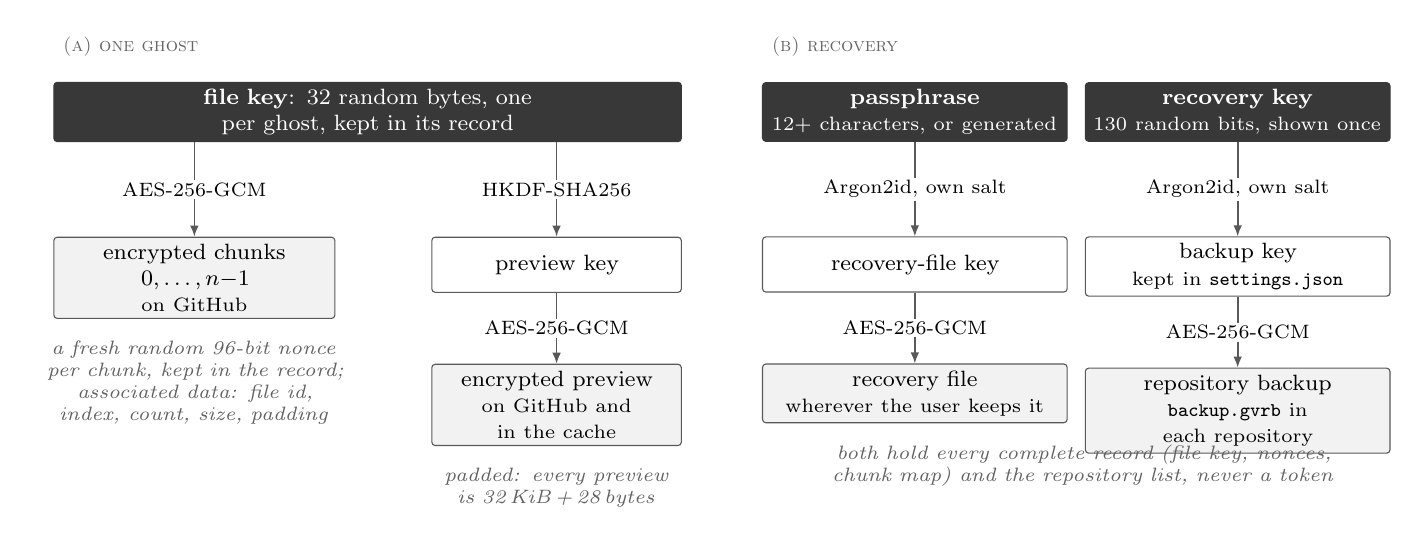
\begin{tikzpicture}[
  font=\footnotesize,
  box/.style={draw=black!65, fill=white, rounded corners=1.2pt, align=center, inner sep=2.4pt,
              minimum height=7mm, text width=#1},
  box/.default=30mm,
  dark/.style={box=#1, fill=black!78, draw=black!78, text=white},
  data/.style={box=#1, fill=black!5},
  arr/.style={-{Latex[length=1.4mm,width=1.1mm]}, draw=black!65, semithick},
  how/.style={font=\scriptsize, fill=white, inner sep=1pt, align=center},
  note/.style={font=\scriptsize\itshape, text=black!62, align=center,
              execute at begin node={\hyphenpenalty=10000\exhyphenpenalty=10000}},
  panel/.style={font=\scriptsize\scshape, text=black!60},
]
% ---- (a) one ghost --------------------------------------------------------------------------
\node[dark=78mm] (fk) at (0,0) {\textbf{file key}: 32 random bytes, one per ghost, kept in its record};
\node[data=34mm, below=12mm of fk.south west, anchor=north west] (chunks)
  {encrypted chunks $0,\dots,n{-}1$\\\scriptsize on GitHub};
\node[box=30mm, below=12mm of fk.south east, anchor=north east] (pk) {preview key};
\node[data=30mm, below=9mm of pk] (pv) {encrypted preview\\\scriptsize on GitHub and in the cache};
\draw[arr] (chunks.north |- fk.south) -- node[how] {AES-256-GCM} (chunks.north);
\draw[arr] (pk.north |- fk.south) -- node[how] {HKDF-SHA256} (pk.north);
\draw[arr] (pk) -- node[how] {AES-256-GCM} (pv);
\node[note, below=1.5mm of chunks, text width=40mm]
  {a fresh random 96-bit nonce per chunk, kept in the record; associated data: file id, index,
   count, size, padding};
\node[note, below=1.5mm of pv, text width=34mm] {padded: every preview is 32\,KiB\,+\,28\,bytes};
\node[panel, anchor=south west] at ([yshift=2mm]fk.north west) {(a) one ghost};

% ---- (b) recovery ---------------------------------------------------------------------------
\begin{scope}[xshift=90mm]
\node[dark=37mm] (pp) at (-20.5mm,0) {\textbf{passphrase}\\\scriptsize 12+ characters, or generated};
\node[dark=37mm] (rk) at (20.5mm,0) {\textbf{recovery key}\\\scriptsize 130 random bits, shown once};
\node[box=37mm, below=12mm of pp] (fkey) {recovery-file key};
\node[box=37mm, below=12mm of rk] (bkey) {backup key\\\scriptsize kept in \texttt{settings.json}};
\node[data=37mm, below=9mm of fkey] (file) {recovery file\\\scriptsize wherever the user keeps it};
\node[data=37mm, below=9mm of bkey] (bak) {repository backup\\\scriptsize \texttt{backup.gvrb} in each repository};
\draw[arr] (pp) -- node[how] {Argon2id, own salt} (fkey);
\draw[arr] (rk) -- node[how] {Argon2id, own salt} (bkey);
\draw[arr] (fkey) -- node[how] {AES-256-GCM} (file);
\draw[arr] (bkey) -- node[how] {AES-256-GCM} (bak);
\node[note, below=1.5mm of file.south east, anchor=north, xshift=2mm, text width=70mm]
  {both hold every complete record (file key, nonces, chunk map) and the repository list,
   never a token};
\node[panel, anchor=south west] at ([yshift=2mm]pp.north west) {(b) recovery};
\end{scope}
\end{tikzpicture}

\caption{The keys. (a) Each ghost has its own random key; its preview key is derived from it, so
chunks and preview never share a key. (b) A recovery bundle holds the records, with their keys,
encrypted under a key derived from a passphrase or a generated recovery key; each bundle key has
its own random salt. Black: secrets that are generated or chosen, never derived.}
\label{fig:keys}
\end{figure*}

\subsection{Keys}\label{sec:keys}
\figref{fig:keys} shows the keys and \tabref{tab:sizes} their sizes. A \emph{file key} is 32 bytes
from the operating system's random source (Python's \path{secrets.token_bytes}), one per ghost, stored in
its record. It encrypts that ghost's chunks and nothing else. The \emph{preview key} is
HKDF-SHA256 of the file key with the label \path{ghostvault/v6/subkey/preview}; it is derived when
needed and never stored. The keys of recovery bundles are derived with Argon2id from a passphrase
or a recovery key, each with its own random 16-byte salt (\secref{sec:recovery}).

Keys at rest are plain base64 in the records and settings, in files only the user can read. This is
deliberate. Wrapping them with a key kept in the operating system's keychain would protect nothing
against malware running as the user, which can read the keychain too, and losing that one keychain
entry would lose every ghost at once. The protection for a stolen computer is full-disk encryption;
backups of the data folder contain the keys and must be protected like it.

\subsection{Chunks}\label{sec:chunks}
A file is read in chunks of 512\,KiB of plaintext; a file of $s$ bytes has $\lceil s/524\,288
\rceil$ chunks, so an empty file has none. Each chunk is encrypted on its own with AES-256-GCM
under the file key and a fresh random 96-bit nonce; the ciphertext is the plaintext followed by a
16-byte tag. The nonce stays in the record; GitHub stores only the ciphertext.

Each chunk's associated data (\lstref{lst:aad}) names the file, the chunk's position, the number of
chunks, the file's exact size and whether the last chunk is padded. A chunk therefore cannot be
moved into another file, to another position, or into a file with more or fewer chunks without
failing authentication, and the size and padding flag in a record cannot be changed without every
chunk failing. The length used to strip the padding is thus authenticated, not taken on trust from
the record.

\begin{lstlisting}[basicstyle=\ttfamily\scriptsize,caption={Associated data of a chunk;
\code{p} or \code{u} says whether the last chunk is padded.},label={lst:aad}]
ghostvault/v6/<file id>/<index>/<count>/<size>/<p|u>

ghostvault/v6/5ada355b920792c5ba14be70737ffc5a/9/10/4860280/p
\end{lstlisting}

Nonces are random, and every encryption under a key uses a fresh one. With random 96-bit nonces,
NIST limits a key to $2^{32}$ encryptions~\cite[Sec.~8.3]{nist-gcm}. A file key is used once per
chunk of one file (a file of 1\,TiB has $2^{21}$ chunks), a preview key once or a few times, a
recovery-file key once, and the backup key once per backup version, so every key stays many orders of magnitude
below that limit.

Records written by earlier versions of GhostVault (record format 5) bind the file, the position and
the count, as \path{ghostvault/v4/<file id>/<index>/<count>}. They are still read, and restored
with that associated data; new records always use the form above.

\subsection{Padding}\label{sec:padding}
By default (\emph{Enhanced privacy} in the window), the last chunk's plaintext is filled with
random bytes up to the full 512\,KiB before it is encrypted, so every chunk of a ghost has the same
ciphertext size, 524\,304 bytes. No chunk is ever added: a file whose size is a multiple of 512\,KiB
is unchanged, and an empty file has no chunks. Restoring decrypts each chunk, checks its length,
and keeps exactly the recorded size. Each ghost records whether it was padded, and \emph{Storage
efficiency} turns padding off for new ghosts. \tabref{tab:padding} shows what GitHub stores.

\begin{table}[t]
\caption{Bytes of chunk ciphertext stored on GitHub}\label{tab:padding}
\centering\footnotesize
\begin{tabular}{@{}rrrr@{}}
\toprule
\textbf{File size (bytes)} & \textbf{Chunks} & \textbf{Padded} & \textbf{Not padded} \\
\midrule
0 & 0 & 0 & 0 \\
1 & 1 & 524\,304 & 17 \\
102\,400 & 1 & 524\,304 & 102\,416 \\
524\,288 & 1 & 524\,304 & 524\,304 \\
524\,289 & 2 & 1\,048\,608 & 524\,321 \\
5\,242\,881 & 11 & 5\,767\,344 & 5\,243\,057 \\
\bottomrule
\end{tabular}

\vspace{2pt}\raggedright\scriptsize Measured with \code{tools/measure.py}; each chunk adds a 16-byte
tag. Padded, every chunk is 524\,304 bytes.
\end{table}

Padding hides a file's exact size, not its approximate size: GitHub still sees the chunk count,
which gives the size to within 512\,KiB. The cost is at most 512\,KiB per ghost on GitHub.

\subsection{Checks on restore}\label{sec:checks}
A restore accepts a chunk only after five checks, all done before anything is written under the
file's final name:
\begin{enumerate}
\item the Git blob id is recomputed from the downloaded bytes and must equal the recorded id;
\item the SHA-256 of the ciphertext must equal the one recorded at upload;
\item the GCM tag must verify, with the associated data above;
\item for records of format 6, the plaintext length must be exactly what the recorded size and
padding imply;
\item after the last chunk, the whole file's SHA-256 must equal the original's.
\end{enumerate}
Git's ids are SHA-1 hashes. GhostVault uses them to name and find what GitHub stores and to detect
damage, not to resist an adversary: integrity against an adversary rests on the GCM tag and the
SHA-256 checks.

\subsection{Previews}\label{sec:previews}
For an image (JPEG, PNG, GIF, WebP or BMP, recognised by extension and decoded only in those
formats), GhostVault makes a preview of at most 200\,$\times$\,150 pixels, encoded as JPEG in at
most 32\,KiB\,$-$\,4 bytes. Decoding is bounded: images over 50 megapixels are refused from their
header, before any pixel is read, and JPEGs are decoded at reduced scale. The preview is encrypted
as soon as it exists and is never written in plaintext:
\begin{align*}
  \mathit{blob} = n \,\|\, \mathrm{AES\text{-}GCM}_{k_p}\bigl(&n,\; \ell \,\|\, \mathit{image} \,\|\,
  \mathit{pad},\\ &\text{``}\texttt{ghostvault/v6/preview/}\mathit{id}\text{''}\bigr),
\end{align*}
where $k_p$ is the preview key, $n$ a fresh 12-byte nonce, $\ell$ the image length in four bytes,
and the random padding brings the plaintext to 32\,KiB. Every preview blob therefore has the same
size, 32\,KiB plus 28 bytes. It is uploaded under its own random path to the repository of the
ghost's first chunk, committed with the chunks, and kept in a local cache in the same encrypted
form; it is decrypted in memory to be shown. Hiding a ghost's preview deletes only the local copy.
A preview reveals that a ghost has one, and nothing else.

\begin{table}[t]
\caption{Fixed sizes and parameters}\label{tab:sizes}
\centering\footnotesize
\begin{tabular}{@{}lr@{}}
\toprule
\textbf{What} & \textbf{Value} \\
\midrule
file key, preview key, bundle keys & 32 bytes \\
nonce, for every encryption & 12 bytes \\
authentication tag & 16 bytes \\
chunk plaintext & 524\,288 bytes \\
chunk ciphertext, padded & 524\,304 bytes \\
preview blob & 32\,796 bytes \\
file id & 16 random bytes (32 hex) \\
chunk path & \code{ghostvault/<2 hex>/<32 hex>.bin} \\
Argon2id: memory, passes, lanes & 256\,MiB, 3, 4 \\
scrypt fallback: $N$, $r$, $p$ & $2^{17}$, 8, 1 \\
bundle salt & 16 bytes \\
bundle padding unit & 64\,KiB \\
recovery key & 130 bits + 2 check characters \\
\bottomrule
\end{tabular}
\end{table}

\section{Local State and the Journal}\label{sec:state}

\subsection{The data folder}\label{sec:folder}
All local state is in one folder, the per-user application-data folder of each system:
\begin{itemize}
\item Windows: \code{\%LOCALAPPDATA\%\textbackslash GhostVault}, which is local, not roaming, so the keys
do not travel with a roaming profile;
\item macOS: \path{~/Library/Application Support/GhostVault};
\item Linux: \path{$XDG_DATA_HOME/ghostvault}, or \path{~/.local/share/ghostvault}.
\end{itemize}
\lstref{lst:folder} shows its contents. On Linux and macOS, folders are created with mode 0700 and
files with 0600; on Windows the folder inherits the per-user permissions of the profile.

\begin{lstlisting}[caption={The data folder (modes on Linux and macOS).},label={lst:folder}]
<data folder>/              0700
  settings.json             0600  repositories, options
  manifests/<file id>.json  0600  one record per ghost
  thumbs/<file id>.gvp      0600  encrypted previews
  logs/ghostvault.log       0600  file ids, never names
  damaged/                  0700  unreadable files, kept
  vault.lock                0600  held while running
\end{lstlisting}

Nothing is staged on disk: chunks are encrypted and uploaded one at a time, and restored chunks go
straight into the hidden output file. Nothing in the folder records the folder's own location, so it
can be moved or restored from a backup. While GhostVault runs, it holds an exclusive lock on
\code{vault.lock} (\code{flock}, or \code{msvcrt.locking} on Windows); the operating system releases
it when the process ends, however it ends, and a second instance on the same folder is refused.

\subsection{Records}\label{sec:records}
Each ghost is one JSON record, \lstref{lst:record}, named after its random 128-bit file id. A record
is validated every time it is read: its shape, its version (5 or 6), and every value used to build a
request, choose a path or delete something must have the only form GhostVault creates: owner and
repository names, the base folder, chunk and preview paths, blob ids, nonces, the key length, the
cipher and associated-data label, the name of a temporary restore file and of the hidden name the
original is moved to, each beside its file. Records of format 6 must also have a chunk count that
matches their size. A record that fails is shown as damaged and left untouched; nothing acts on it,
and it affects no other ghost.

\begin{lstlisting}[language=gvjson,caption={A record of a ghost with ten chunks, abridged; the
values are from a real run against the simulated GitHub.},label={lst:record}]
{"format": "ghostvault-manifest", "version": 6,
 "fileId": "5ada355b920792c5ba14be70737ffc5a",
 "state": "ready", "displayName": "harbour.png",
 "original": {"name": "harbour.png", "size": 4860280,
   "path": "...", "sha256": "f9b10964...932b14",
   "mode": 420, "atimeNs": ..., "mtimeNs": ...,
   "identity": {"dev": ..., "ino": ..., "size": 4860280,
                "mtime_ns": ...}},
 "crypto": {"cipher": "AES-256-GCM",
            "key": "owrw+KXo...6508=",
            "aad": "ghostvault/v6"},
 "chunkSize": 524288, "padding": true,
 "chunks": [{"index": 0, "repo": "d825332f29363c8d",
   "path": "ghostvault/78/7e34107f...6b144794.bin",
   "plainSize": 524288, "nonce": "VG7sZuNj9KNv8fQb",
   "cipherSha256": "27b4368a...4e85e8",
   "blobSha": "b295c74a...616173be52d5"}, ...],
 "repos": {"d825332f29363c8d": {"owner": "alice",
   "repo": "vault1", "baseFolder": "ghostvault",
   "committed": true, "deleted": false}, ...},
 "preview": {"enabled": true, "remote": {"repo": ...,
   "path": "ghostvault/9c/962063f7...7c65b415.bin",
   "blobSha": ..., "committed": true}},
 "placement": {"strategy": "distributed",
               "eligible": 2, "repositories": 2},
 "notes": [], "restore": null}
\end{lstlisting}

\subsection{Durable writes}\label{sec:durable}
Every state file is written the same way: a new owner-only file is created beside the target
(\code{O\_EXCL}, \code{O\_NOFOLLOW}), written and flushed to disk, renamed over the old file, and
then the folder is flushed. After a crash the file holds either its old or its new content; a
leftover temporary file is removed at the next start. \tabref{tab:durable} lists what each step
means on each system. Flushing a file on macOS uses \code{F\_FULLFSYNC}, because \code{fsync} there
does not flush the drive's cache; Windows cannot flush a folder, so renames there are issued with
\code{MOVEFILE\_WRITE\_THROUGH}, which returns only once the rename is on disk. All of this uses
the standard library (\code{os}, \code{fcntl}, \code{msvcrt}, \code{ctypes}); no shell command is run.

\begin{table}[t]
\caption{Durability on each system}\label{tab:durable}
\centering\footnotesize
\setlength{\tabcolsep}{4pt}
\begin{tabular}{@{}L{17mm}L{17mm}L{19mm}L{24mm}@{}}
\toprule
\textbf{Step} & \textbf{Linux} & \textbf{macOS} & \textbf{Windows} \\
\midrule
flush a file & \code{fsync} & \code{F\_FULLFSYNC} & \code{FlushFileBuffers} \\ \addlinespace[1.6pt]
flush a folder & \code{fsync} & \code{F\_FULLFSYNC} & not possible; renames written through \\ \addlinespace[1.6pt]
replace a file & \code{rename} & \code{rename} & \code{MoveFileExW}, replace and write-through \\ \addlinespace[1.6pt]
publish without replacing & hard link & hard link & \code{MoveFileExW} without replace \\ \addlinespace[1.6pt]
lock & \code{flock} & \code{flock} & \code{msvcrt.locking} \\
\bottomrule
\end{tabular}
\end{table}

\subsection{The journal}\label{sec:journal}
A record's \code{state} is the journal of the operation in progress (\figref{fig:journal}). It is
written durably before every step that changes something outside the data folder, and every
irreversible step is preceded by a state that tells start-up recovery how to finish or undo it.
The code marks each such point with a named checkpoint; the tests stop the process at every one of
them (\secref{sec:verification}).

\begin{figure}[t]
\centering
% Fig.: the journal states of one ghost record and the transitions between them.
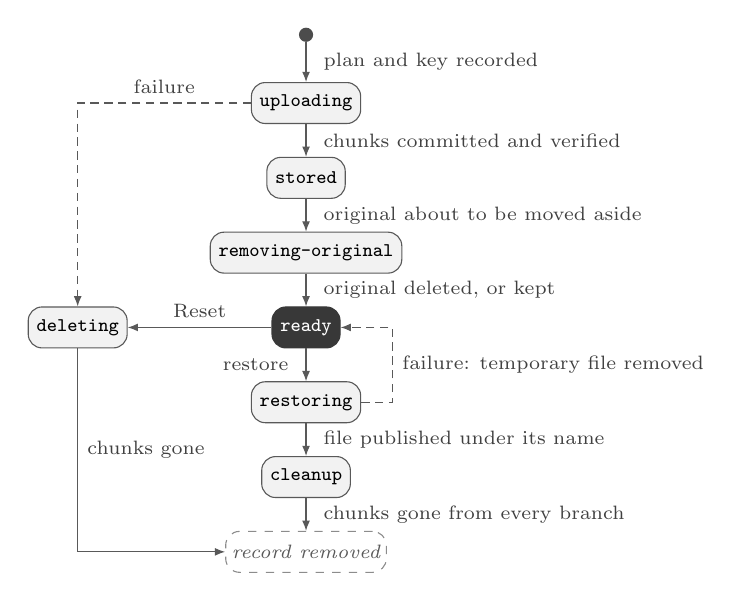
\begin{tikzpicture}[
  font=\scriptsize,
  st/.style={draw=black!65, fill=black!5, rounded corners=5pt, inner xsep=3pt, inner ysep=2.2pt,
             font=\scriptsize\ttfamily, minimum height=5.2mm},
  ok/.style={st, fill=black!78, draw=black!78, text=white},
  gone/.style={draw=black!45, dashed, rounded corners=5pt, inner sep=2.2pt, font=\scriptsize\itshape,
               text=black!65, minimum height=5.2mm},
  arr/.style={-{Latex[length=1.3mm,width=1mm]}, draw=black!65},
  fail/.style={arr, densely dashed},
  lab/.style={font=\scriptsize, text=black!75, align=left,
              execute at begin node={\hyphenpenalty=10000}},
]
\def\step{9.5mm}
\node[st] (up) at (0,0) {uploading};
\node[st, below=\step of up.center, anchor=center] (stored) {stored};
\node[st, below=\step of stored.center, anchor=center] (rem) {removing-original};
\node[ok, below=\step of rem.center, anchor=center] (ready) {ready};
\node[st, below=\step of ready.center, anchor=center] (res) {restoring};
\node[st, below=\step of res.center, anchor=center] (clean) {cleanup};
\node[gone, below=\step of clean.center, anchor=center] (gone) {record removed};
\node[st] (del) at (-29mm, 0 |- ready) {deleting};

\fill[black!70] ([yshift=6mm]up.north) circle (0.9mm) coordinate (start);
\draw[arr] ([yshift=5.1mm]up.north) -- node[lab, right=1mm] {plan and key recorded} (up);
\draw[arr] (up) -- node[lab, right=1mm] {chunks committed and verified} (stored);
\draw[arr] (stored) -- node[lab, right=1mm] {original about to be moved aside} (rem);
\draw[arr] (rem) -- node[lab, right=1mm] {original deleted, or kept} (ready);
\draw[arr] (ready) -- node[lab, left=1mm] {restore} (res);
\draw[arr] (res) -- node[lab, right=1mm] {file published under its name} (clean);
\draw[arr] (clean) -- node[lab, right=1mm] {chunks gone from every branch} (gone);

\draw[fail] (up.west) -| node[lab, pos=0.25, above] {failure} (del.north);
\draw[arr] (ready.west) -- node[lab, above] {Reset} (del.east);
\draw[arr] (del.south) |- node[lab, pos=0.25, right] {chunks gone} (gone.west);
\draw[fail] (res.east) -- ++(4mm,0) |- node[lab, pos=0.25, right] {failure: temporary file removed} (ready.east);
\end{tikzpicture}

\caption{The journal states of a record. Solid arrows are the normal course of an operation;
dashed arrows are taken on failure. An interruption in any state is handled at the next start as
\tabref{tab:recovery} describes.}
\label{fig:journal}
\end{figure}

At every start GhostVault runs this recovery first, as an operation of its own during which the
window accepts no other: it removes leftover temporary files, checks the settings, handles each
record by its state (\tabref{tab:recovery}), and tells the user what it did. The rules
for \state{stored} and \state{removing-original} are written so that a file found at the original's
path is never called the original unless its identity is the uploaded file's: a new file saved under
the same name is not the user's original, and saying so could lead the user to delete it.

\begin{table}[t]
\caption{Start-up recovery by journal state}\label{tab:recovery}
\centering\footnotesize
\begin{tabular}{@{}L{24mm}L{58mm}@{}}
\toprule
\textbf{State} & \textbf{What the next start does} \\
\midrule
\state{uploading} & the record becomes \state{deleting}: every path it lists is removed from the
branches, then the record; the original was never touched \\ \addlinespace[1.6pt]
\state{deleting} & removal from GitHub is finished, then the record is removed \\ \addlinespace[1.6pt]
\state{stored} & the ghost is complete; the original is kept, and the user is told whether the
file at its path is still the original \\ \addlinespace[1.6pt]
\state{removing-original} & if the file under the hidden name exists, it is checked again and
deleted if it is the uploaded file, put back otherwise; the ghost is complete either way \\ \addlinespace[1.6pt]
\state{restoring} & the temporary file is removed; if the final file is in place and matches the
original's SHA-256, it is adopted and clean-up continues, otherwise the ghost is \state{ready}
again \\ \addlinespace[1.6pt]
\state{cleanup} & removal from GitHub is retried; while GitHub cannot be reached it stays pending,
with a Retry button \\
\bottomrule
\end{tabular}
\end{table}

\emph{Unreferenced blobs.} If ghosting is interrupted after some chunks were uploaded but before
they were committed, those blobs exist in the repository's object store without being on any
branch. They are encrypted and listed nowhere, and Git removes unreferenced objects eventually, on
GitHub's schedule. GhostVault cannot delete a blob directly: the Git Data API has no such
operation.

\subsection{Damage}
An unreadable record is shown as damaged and never overwritten, and it pauses backups until the
user resolves it (\secref{sec:incomplete}). An unreadable settings file is moved into
\code{damaged/} and GhostVault starts with empty settings; ghosts are unaffected, because every
record names its own repositories.

\section{Ghosting a File}\label{sec:ghost}

\subsection{Accepting the original}
GhostVault accepts only a regular file with a single name. Symbolic links, folders, devices, pipes
and sockets are refused, and so are Windows symbolic links and mount points; a file with more than
one hard link is refused because its data would stay on disk under the other name after
GhostVault removed this one; and nothing inside the data folder can be ghosted. The file is opened
once, without following links (\code{O\_NOFOLLOW}, \code{O\_NONBLOCK}), and the identity of the open
file (device, inode, size, modification time) must match that of the path, so a file replaced at
the moment of opening is refused.

Everything is read through that one handle. The size recorded is the number of bytes actually read,
and after the last chunk the file's size and modification time are compared with those at opening.
If anything changed, nothing is committed and the partial upload is undone. On Windows the handle
is opened with Python's default sharing, which does not include deletion, so while the upload runs
Windows refuses to rename, replace or delete the original; writing into it remains possible and is
detected.

\subsection{The plan}
Before anything is sent, GhostVault draws a random file id and a random key, decides where every
chunk goes, and gives every chunk, and the preview if there is one, a random path of the form
\code{ghostvault/<2 hex>/<32 hex>.bin}. Placement follows one of two strategies, chosen in Settings
or for a single file:
\begin{itemize}
\item \emph{distributed} (the default): the eligible repositories are put in a random order and dealt
chunks in turn, so each of $r$ repositories holds $\lfloor n/r\rfloor$ or $\lceil n/r\rceil$ of a file's
$n$ chunks;
\item \emph{consolidated}: every chunk goes to one eligible repository, chosen at random.
\end{itemize}
Neither strategy is redundancy: every chunk is stored once. A distributed file needs every
repository that holds one of its chunks; a consolidated file needs one repository, which holds all
of it. The record lists the repository of every chunk, and every later operation works from that
list, so changing the setting never moves an existing ghost. With a single eligible repository,
distributed placement cannot distribute; the record and the result message say so.

The plan, the key and the original's identity are then written as the record, in state
\state{uploading}, before the first request (\figref{fig:lifecycle}). From that moment every path the
ghost could ever create on GitHub is known to the journal.

\subsection{Upload and commit}
Blobs can be created only in a repository that has a commit, so an empty repository is first
initialised with an empty file, \code{ghostvault/.keep}. Then the file is streamed: each chunk is
read, padded if it is the last, encrypted, hashed (SHA-256 and its Git blob id), and uploaded as a
blob. Git derives a blob's id from the bytes it holds~\cite{git-objects}, so the id in GitHub's
reply must equal the one computed locally. Only one chunk is held in memory at a time, and nothing is written to disk. A
blob is part of no branch until a commit refers to it, so an interrupted upload leaves only
unreferenced, encrypted objects.

Once every chunk is uploaded, every blob id is written to the record, and only then is anything
committed. Each repository gets one commit: a tree built on the branch's current tree with the new
paths, a commit with the branch head as its parent and the message \code{Update}, and a branch
update that must be a fast-forward. If a commit fails without a clear answer, GhostVault reads the
branch to see what arrived before deciding (\secref{sec:uncertain}).

\subsection{Verification before deletion}\label{sec:verify}
Before the original may be deleted, three things must hold for every repository used:
\begin{enumerate}
\item each blob id was computed locally from the exact ciphertext, and GitHub answered the upload
with the same id;
\item the branch, read again from its head, maps every recorded path to exactly that blob id. Git ids
are content hashes, so this establishes that the branch refers to exactly the uploaded bytes, for
every chunk. A path that is not yet listed is looked for again after 1, 2 and 4\,s, because a read
may be served by a replica that has not caught up; still missing, the ghost fails and is undone;
\item the first chunk and one other chunk chosen at random are downloaded through the same request a
restore uses, and their SHA-256 must equal the uploaded ciphertext's. This shows that the data can be
read back with the current token, not only that it is referenced.
\end{enumerate}
Downloading every chunk again would double the transfer for little more assurance, since the second
check already covers every chunk and GitHub checks object ids itself. What no check made at this
time can rule out is damage or loss on GitHub's side afterwards. The record then moves to
\state{stored}.

\subsection{Removing the original}\label{sec:remove}
Checking a path and then deleting the same path would leave a window in which another program, an
editor saving by rename for example, replaces the file, and the newer file, which was never
uploaded, would be deleted. GhostVault therefore moves the original aside before checking it
(\lstref{lst:remove}). From the rename on, whatever appears under the original's name is never
touched.

\begin{lstlisting}[caption={Removing the original, once the record says \state{removing-original}.},
label={lst:remove}]
file at the path not the uploaded one?    keep it
  (device, inode, size, mtime)
hidden = ".<name>.<12 random hex>.ghostvault-removing"
record hidden in the record (durably)
rename path -> hidden          (atomic, same folder)
open hidden    (Windows: no sharing but reading)
  identity changed?            put back, keep
  SHA-256 != uploaded?         put back, keep
  size or mtime changed now?   put back, keep
  delete     (POSIX: unlink, if hidden still names
              the open file; Windows: by the handle)
put back = publish under the old name, never
  replacing; if taken: "<name> (kept by GhostVault)"
\end{lstlisting}

On Windows the hidden file is opened with read and delete access, sharing only reading, and deleted
through that same handle (\code{SetFileInformationByHandle}): no other program can write to it,
rename it or delete it while it is checked, and opening fails if one already has it open for
writing, so the file deleted is exactly the file checked. Linux and macOS offer no way to delete a
file only if nobody else has it open for writing. There, a program that already had the file open
can still write to it in the moment between the last check and the deletion; GhostVault narrows
that window by checking size and modification time once more just before it, and claims no more.

If any step fails, the original is kept, or put back without replacing anything, and the ghost is
completed as \state{ready} with the reason; Windows answers such as ``access denied'' or ``in use''
are handled the same way. The ghost is complete either way: only the deletion of the original was
given up.

\section{Restoring a File}\label{sec:restore}

\subsection{Writing the file}
A restore starts only for a ghost in state \state{ready}, into a folder the user chooses, under a
name that may not exist there and must fit in 255 bytes. The record moves to \state{restoring} and
names the destination and a hidden temporary file beside it,
\code{.<name>.<12\nobreakspace{}hex>.ghostvault-part}, created exclusively and readable by the owner only.

Chunks are downloaded in parallel, eight at a time, with at most sixteen held in memory, and are
written into the temporary file in order. Each is checked as described in \secref{sec:checks}
before it is written, and the first failure stops every further download. After the last chunk the
whole file's SHA-256 is compared with the original's. The file then gets the original's permission
bits (without setuid, setgid or sticky bits) and its access and modification times, or on Windows
its read-only attribute and times, and is flushed to disk. Nothing has a final name yet; a failure
up to here removes the temporary file and leaves the ghost \state{ready}.

\subsection{Publishing without replacing}\label{sec:publish}
The finished file is given its final name in a way that can never replace a file, however recently
that file appeared. On Linux and macOS this is a hard link to the final name, which fails if the
name exists, followed by removal of the temporary name; on file systems without hard links it is
\code{renameat2} with \code{RENAME\_NOREPLACE} (Linux) or \code{renamex\_np} with
\code{RENAME\_EXCL} (macOS), and where neither exists the restore is refused rather than risk an
overwrite. On Windows it is \code{MoveFileExW} without the replace flag and with write-through. If a
file of that name appeared during the restore, it is left untouched, the temporary file is removed,
and the user is asked for another name. The folder is then flushed, and only then does the record
move to \state{cleanup}.

\subsection{Removing the remote copy}
Clean-up removes the ghost's paths from each repository with one commit, then reads the branch again;
the removal is complete only when a fresh listing shows none of them. A round that GitHub refused,
applied only in part, or acknowledged without effect is followed by another, after 2, 4 and 8\,s,
up to four rounds. Rounds can be repeated safely: the paths are random and recorded, absent ones are
skipped, and the branch is never forced. A refusal that repeating cannot fix (a rejected token, a
missing repository, an exhausted rate limit) ends the rounds at once. If paths are still listed after
the last round, the error says how many, with GitHub's last status, message and request id and what
each round sent and saw; the ghost stays in \state{cleanup}, is shown with a Retry button, and is
retried at the next start.

Only when every repository has confirmed the removal are the record and its cached preview deleted.
Before the record is deleted, its id is added to the ghosts GhostVault has removed (when a recovery
file or the repository backup may hold it), so that a later backup can leave it out without the
removal being mistaken for a lost record (\secref{sec:incomplete}).

Removal takes the ghost off the branch. It does not erase it: the commits that added the chunks
remain in the repository's history, and GitHub may keep unreachable objects for a time. A removed
ghost stays unreadable only as long as its key exists nowhere: not in the data folder, not in a
backup of that folder, and not in a recovery bundle made while the ghost existed.

\section{Working with GitHub}\label{sec:github}

GhostVault uses GitHub's REST API, version \code{2022-11-28}: the Git database endpoints (blobs,
trees, commits and references~\cite{gh-git}) for all of its data, the Contents API only to give an
empty repository its first commit and to look paths up one by one, and the repository endpoint to
check a repository and its permissions.

\subsection{Repositories and tokens}\label{sec:gh-checks}
A repository is added with its address (only \code{github.com} is accepted) and a token. GhostVault
accepts it only if GitHub describes it as private, not archived, and writable with that token
(\code{permissions.push}); a fine-grained token needs \emph{Contents: read and write} on it. When,
during an operation, GitHub rejects the token (401, 403) or no longer shows the repository, the
repository is marked as failing in Settings and new ghosts avoid it. A 404 for a branch is taken to
mean an empty repository only if the repository itself still answers, so a repository that has
become inaccessible is never mistaken for an empty one.

Tokens are kept in the operating system's keychain through the \code{keyring} library, which is
restricted to backends that store secrets in an operating-system keychain: Windows Credential
Manager, the macOS Keychain, Secret Service (libsecret) and KWallet. Plaintext or file-based backends
are never used, even when installed, and \code{keyring}'s fall-through chain is bypassed, so a
failing keychain can never fall through to a file. Without a usable keychain, tokens are kept in
memory for the session. Tokens never appear in GhostVault's files or log, and GitHub's own error
messages, where they are logged or kept in a record's notes, pass through a filter that removes
anything shaped like a token.

\subsection{Transport}
Requests go over one persistent HTTPS connection per thread to \code{api.github.com}, so a TCP and
TLS handshake is not paid per request. A proxy configured in the environment is honoured, with its
credentials, by tunnelling through it. Certificates are verified against the operating system's
trust store through \code{truststore}~\cite{truststore}, so certificate authorities installed by the
system or an organisation are trusted exactly as the system's browser trusts them; one TLS context is
passed explicitly to every request, and Python's process-wide defaults are never changed. Redirects
for renamed repositories are followed (301 and 302 for reads, 307 and 308 for any request), never to
another host and at most three in a row. A reply larger than 128\,MiB is not read.

Before an operation, a four-second check asks GitHub's \code{/rate\_limit} endpoint, authenticated
with a token, whether GitHub can be reached. An answer counts only if it comes from GitHub: a proxy
asking for a login, a sign-in page or filter answering in GitHub's place (no GitHub request id), and
a certificate that is not GitHub's are each reported as such instead of being taken for ``online''.

\subsection{Retries, rate limits and pacing}
Every request passes through one retry layer per vault (\tabref{tab:retries}). Rate limits are
waited out rather than treated as failures: a large upload can meet GitHub's limits, and waiting is
better than undoing hours of work. The window's progress line says until when it waits.

\begin{table}[t]
\caption{What the retry layer does}\label{tab:retries}
\centering\footnotesize
\begin{tabular}{@{}L{24mm}L{56mm}@{}}
\toprule
\textbf{Situation} & \textbf{What happens} \\
\midrule
no reply; 500, 502, 503, 504 & retried, if safe to repeat: at most 6 tries, exponential backoff with
full jitter (1, 2, 4\,s \dots, at most 60\,s) \\ \addlinespace[1.6pt]
429, or 403 with rate-limit signs & waited out: \code{Retry-After} (seconds or an HTTP date), else
until \code{X-RateLimit-Reset}, else 1, 2, 4 \dots 15 minutes; a single wait over 65 minutes, or
3 hours of waiting for one request, is reported instead \\ \addlinespace[1.6pt]
other 4xx & not retried: it describes a real problem \\ \addlinespace[1.6pt]
any write & serialised, at least 1\,s after the previous write \\
\bottomrule
\end{tabular}
\end{table}

GitHub asks integrators to make requests serially rather than concurrently, and to wait at least one
second between write requests~\cite{gh-best}. GhostVault serialises all writes and spaces them at
least one second apart. Downloads during a restore are reads and run up to eight at a time: below
GitHub's limit of 100 concurrent requests~\cite{gh-rate}, but not strictly serial; a rate-limit reply
to any of them is waited out like any other.

\subsection{Uncertain outcomes}\label{sec:uncertain}
Every read, and creating a blob, a tree or a commit, is safe to repeat: blobs are content-addressed,
and trees and commits are unreferenced until a branch points at them. Moving a branch and creating a
file through the Contents API are not. When one of those fails without a reply, or with an error
that does not say whether it took effect, the outcome is \emph{uncertain}, and GhostVault reads the
branch to find out: if it points at the new commit, the change happened; if it is unchanged, the
update is sent again (it can only fast-forward, so repeating it is safe); if someone else moved it,
the commit is rebuilt on top of the new head. A reply that names a different commit than the one
sent is resolved the same way. If GitHub refuses a tree because its base no longer holds a path being
deleted (a 422), the branch is read again and the commit rebuilt from it. A branch is never forced,
so another writer's commits to the same repository are never overwritten.

\subsection{Large repositories}
Listing a branch reads its tree recursively. GitHub truncates a recursive listing beyond 100\,000
entries or 7\,MB~\cite{gh-git}; GhostVault then looks each path it needs up on its own instead, which
is slower but correct. A repository of the size GitHub recommends, ``ideally less than 1\,GB, and
less than 5\,GB is strongly recommended''~\cite{gh-large}, holds at most about ten thousand chunks,
far below the point where listings are truncated.

\section{Recovery}\label{sec:recovery}

A ghost's key and chunk map exist only in its record. Losing the data folder, or the computer,
would therefore lose every ghost, although its chunks are still on GitHub. GhostVault offers two
ways to keep the records elsewhere, both encrypted in one format: \emph{recovery files}, written on
request to a place the user chooses, and the \emph{repository backup}, kept up to date automatically
in the repositories if the user turns it on. \tabref{tab:loss} summarises what each kind of loss
costs.

\begin{table}[t]
\caption{What a loss costs}\label{tab:loss}
\centering\footnotesize
\begin{tabular}{@{}L{19mm}L{30mm}L{30mm}@{}}
\toprule
\textbf{Lost} & \textbf{Without a bundle} & \textbf{With a recovery file or the backup} \\
\midrule
one record & that ghost & restored from the bundle \\ \addlinespace[1.6pt]
the data folder or the computer & every ghost & every ghost in the bundle \\ \addlinespace[1.6pt]
the settings & repositories must be added again; ghosts unaffected & the same \\ \addlinespace[1.6pt]
a token & nothing: enter a new one & the same \\ \addlinespace[1.6pt]
a repository & every ghost with a chunk in it & the same: a bundle holds keys, not data \\ \addlinespace[1.6pt]
the passphrase or recovery key & --- & that bundle, for good: there is no reset \\
\bottomrule
\end{tabular}
\end{table}

\subsection{The bundle format}
A bundle (\lstref{lst:bundle}) is a fixed first line, a header of one line of JSON, and the
ciphertext. The payload holds every complete ghost's record, normalised to \state{ready}, and the
repository list without tokens; it holds no previews, log or journal notes. Ghosts whose remote copy
is incomplete or being removed are left out. The key is derived from the secret with Argon2id,
256\,MiB, 3 passes and 4 lanes: the second recommended setting of RFC~9106~\cite{rfc9106} with four
times its memory. Where the \code{cryptography} build has no Argon2id, scrypt with $N=2^{17}$, $r=8$,
$p=1$ is used. The parameters are read from the header and capped (at most 2\,GiB, 20 passes,
16 lanes), so a malicious file cannot make GhostVault allocate unbounded memory, and the whole header
is authenticated as associated data. The plaintext is padded to a multiple of 64\,KiB, so a bundle's
size shows roughly, not exactly, how many ghosts it holds.

\begin{lstlisting}[caption={A recovery bundle; the header is shown wrapped.},label={lst:bundle}]
GHOSTVAULT-RECOVERY\n
{"check":"<8-byte HMAC, base64>","cipher":"AES-256-GCM",
 "format":"ghostvault-recovery","kdf":{"name":"argon2id",
 "iterations":3,"lanes":4,"memoryKiB":262144,
 "salt":"<16 bytes, base64>"},"kind":"file",
 "nonce":"<12 bytes, base64>","version":1}\n
AES-256-GCM(key, nonce,
  length (8 bytes) || payload JSON
    || random padding to a multiple of 64 KiB,
  associated data = the two lines above)
\end{lstlisting}

The \code{check} value is the first eight bytes of HMAC-SHA256 under the derived key. It lets
GhostVault tell a wrong passphrase from a damaged file, and lets an attacker test a guess no faster
than decrypting would. Nothing can open a bundle whose secret is lost.

\subsection{Recovery files}
A recovery file is protected by a passphrase of at least 12 characters, or by one GhostVault
generates. It is written under a temporary name in the chosen folder, flushed, read back and
decrypted to check it, and only then given its name, without replacing an existing file unless the
user confirmed. Importing one validates every record exactly like a local one before anything is
written, so a bundle with one malformed record imports nothing. Repositories not yet configured are
added without a token and marked as needing one. A ghost already present is skipped, and one with the
same id but a different record is reported and not imported, so local records are never replaced.
GhostVault tracks which ghosts are in any recovery file, and Settings shows how many are in none.

\subsection{The repository backup}
Turning the backup on generates a \emph{recovery key}: 26 characters drawn at random from Crockford's
base32 alphabet~\cite{crockford} (130 bits) and two check characters that catch typing errors, shown
in seven groups of four. It is shown once and stored nowhere; the user writes it down. GhostVault
derives the backup key from it once, with Argon2id and a random salt, and keeps the derived key in its
settings, so later backups need no slow derivation. After every change (a ghost added or removed,
renamed, a preview hidden or shown, an import) it writes a new version of the bundle, of kind
\code{repository}, to \code{ghostvault/recovery/backup.gvrb} in every usable repository.

The bookkeeping survives crashes because nothing about it is kept only in memory. Each version's
sequence number is reserved durably before anything is sent. A version is recorded as verified, with
a digest of its content and the ids it holds, only after the branch of each repository it was
written to has been read back and holds exactly the uploaded bytes; a repository that missed it
keeps the backup due. Whether a backup is \emph{due} is computed by comparing that digest with the
current records, so a crash before, during or after a push leaves it due, and the next operation or
start pushes it. A ghost counts as protected by the backup only if it is in the
last verified version. A failed backup is shown in Settings and retried; it never fails the change
that caused it. On a new computer the user adds the repositories with tokens and enters the recovery
key; GhostVault takes the version with the highest sequence number found in any repository.

The backup has a cost. Anyone who can read the repositories holds the ciphertext and, in the
backup, the encrypted keys, so their safety rests entirely on the recovery key. And Git's history
keeps every earlier version: turning the backup off, or restoring a ghost, removes the current file
from the branch, not the old versions. Whoever later obtains the recovery key and the repository's
history can decrypt the keys of ghosts removed long ago, whose chunks are also still in that history.

\subsection{Incomplete records}\label{sec:incomplete}
A new backup replaces the previous one. If it left out a ghost because that ghost's record could not
be read, the good version on GitHub would be replaced by one without that ghost's key: the encrypted
chunks would remain, and no current backup could open them. GhostVault therefore lets a backup leave a
ghost out only if GhostVault itself removed it, and it records the ids of the ghosts it removes before
deleting their records. Then:
\begin{itemize}
\item a record that cannot be read, or a record that a backup or recovery file holds but that
GhostVault never removed, stops every backup and every recovery-file export, and the last verified
backup stays as it is;
\item before a repository's backup is replaced, the current one is read and decrypted; if it holds
ghosts this computer does not know (another computer, an older copy of the data folder), it is not
replaced in any repository, and one this computer cannot open is not replaced either, unless the user
chose to replace it when turning the backup on;
\item the user resolves the situation explicitly: by repairing the records from the backup or a
recovery file (an unreadable record is moved to \code{damaged/}, never deleted), or by setting them
aside, in which case the backup carries their last good records forward.
\end{itemize}
Ghosting and restoring go on working meanwhile; only backups and exports pause, and the window says
why. One case remains open: a repository that cannot be read when a new version is written is not
compared, so if it alone held a newer version made elsewhere, the version written to the other
repositories can supersede it on a new computer.

\section{The Desktop Application}\label{sec:app}

\begin{figure*}[t]
\centering
\begin{tikzpicture}
\node[inner sep=0, draw=black!35] (a) {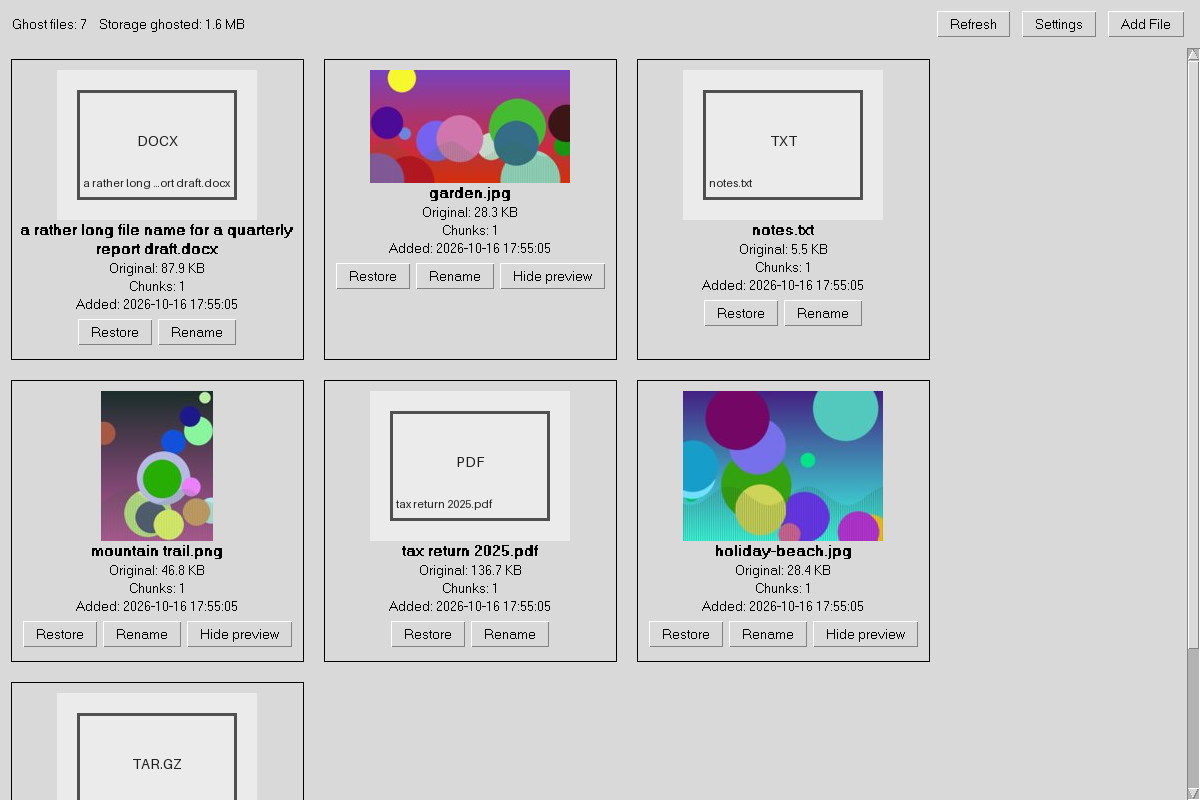
\includegraphics[width=86mm]{images/main-window.png}};
\node[inner sep=0, draw=black!35, right=5mm of a] (b) {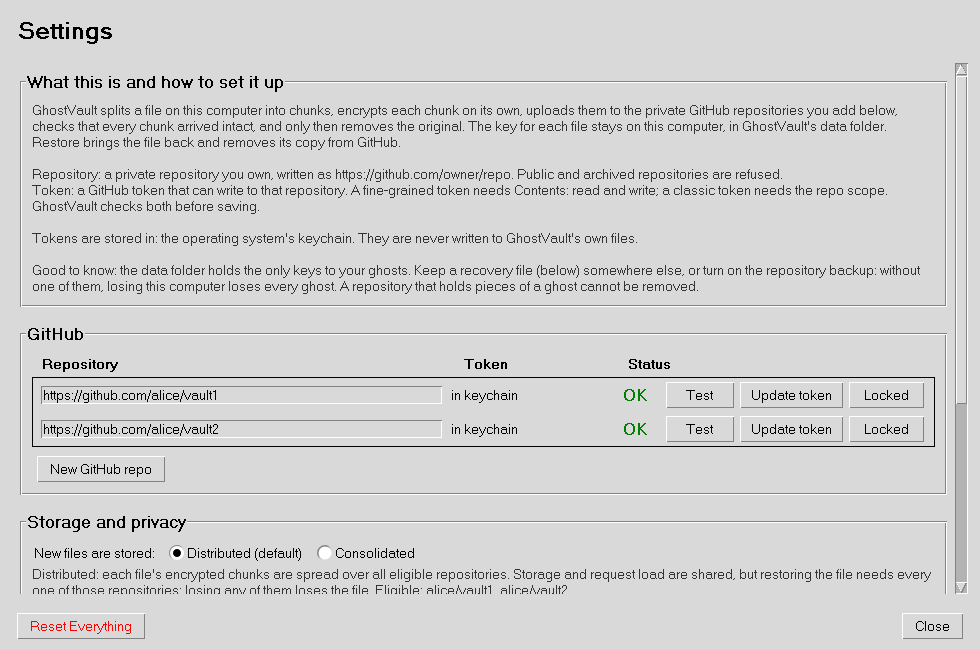
\includegraphics[width=86mm]{images/settings.png}};
\node[font=\footnotesize, below=1.5mm of a] {(a) the main window: one card per ghost};
\node[font=\footnotesize, below=1.5mm of b] {(b) Settings: repositories, storage and privacy, recovery};
\end{tikzpicture}
\caption{The interface, captured against the simulated GitHub with generated sample files. Image
ghosts show their decrypted preview; other files a placeholder drawn in memory. The captures were
made under Xvfb with Tk's X11 core fonts; a desktop with anti-aliased fonts draws the same layout with
smoother text.}
\label{fig:screens}
\end{figure*}

\subsection{The window}
The interface is built from Tk's classic widgets (\figref{fig:screens}). The main window has a bar
with the statistics and three buttons, a progress area that appears while an operation runs, and a
gallery of cards. Settings is a second window with sections for the repositories and their tokens,
storage and privacy (placement, eligible repositories, padding, previews), and recovery. Text worth
copying, such as names, paths, messages and recovery details, can be selected and copied, and every
action can be reached from the keyboard. Every size given in pixels is multiplied by the display's
scale, so the layout keeps its proportions at 125, 150 or 200\,\%; on Windows the process declares
itself DPI-aware so that text is sharp.

\subsection{Work off the window's thread}
Ghosting, restoring, every other operation and every network request run off the window's thread.
An operation that changes the vault runs on a worker thread, one at a time, while the window shows its progress and its
percentage in the title. Small read-only work runs on a pool of two threads: reading a repository's
backup status, and decrypting and decoding previews, except that cached previews are decrypted on the
window's thread for up to 60\,ms per refresh, so that the gallery appears at once. Workers hand their results back through queues that the window thread polls every
60\,ms, and only the window thread touches Tk. If the user closes the window during an operation and
confirms, the process ends at once with the data folder still locked, and the next start finishes or
undoes the operation from its journal, exactly as after a crash; letting the worker continue after
the lock was released could let a second GhostVault act on the same records.

\subsection{Secrets in the interface}
Recovery keys and generated passphrases are shown once, hidden until the user presses \emph{Show},
and copied only by an explicit Copy. A copied secret is taken off the clipboard after one minute and
when GhostVault closes, but only if the clipboard still holds exactly that secret, so anything copied
since is left alone. GhostVault cannot remove copies kept by a clipboard history or a synchronised
clipboard, and the dialog says so. Passphrase and token fields are masked.

\subsection{The log}
The log, \code{logs/ghostvault.log}, is owner-only and rotates at 1\,MB, keeping three old files. It
names ghosts by their ids and repositories by name; it never records the names of the user's files,
keys or tokens. Exceptions are logged by type and place only (file name, line and function of the
innermost frames), never with their message, which can hold a path or a secret; the log's formatter
applies the same rule to any traceback, so no later code can write one in full by mistake.

\subsection{Standalone applications}\label{sec:builds}
Releases contain standalone applications for Windows (x86-64), macOS on Apple silicon and on
Intel, and Linux (x86-64), alongside the Python package (\tabref{tab:release}). Each is a one-folder
PyInstaller~\cite{pyinstaller} build containing Python 3.13, Tcl/Tk and GhostVault's dependencies;
it uses the same data folder as the Python package. One script, \code{packaging/build.py}, builds
locally and in the release workflow, in four steps:
\begin{enumerate}
\item \emph{freeze}: PyInstaller, then license notices generated from the bundled distributions'
metadata, Python's and Tcl/Tk's licenses and, on Linux, the copyright files of the system packages
whose libraries were bundled; then the signature, where configured;
\item \emph{smoke}: the application is started with \code{--version} and \code{--self-check}, which
checks the encryption library, the image decoders, the operating system's certificate store, the
keychain backend and Tk; then its window must open and run for five seconds without logging an
error;
\item \emph{package}: the installer and portable archive, disk image or tar archive;
\item \emph{verify}: the package is unpacked, mounted or installed, and the application in it is
checked again. The Windows installer installs into a scratch folder and uninstalls; on Linux,
\code{install.sh}, an update over it and \code{uninstall.sh} run in a scratch home folder, and the
data folder must come through untouched.
\end{enumerate}
The minimum system of each build is computed from its binaries (the macOS version from the Mach-O
load commands, the glibc version from the ELF symbol versions) and stated in the release notes.

\begin{table}[t]
\caption{Files of a release}\label{tab:release}
\centering\footnotesize
\begin{tabular}{@{}L{29mm}L{51mm}@{}}
\toprule
\textbf{System} & \textbf{File} \\
\midrule
Windows 10 and 11, x64 & installer (Inno Setup; per user by default, without administrator rights)
and portable zip; a windowed \code{GhostVault.exe} and a console \code{ghostvault-cli.exe} \\ \addlinespace[1.6pt]
macOS, Apple silicon & disk image with \code{GhostVault.app} \\ \addlinespace[1.6pt]
macOS, Intel & disk image with \code{GhostVault.app} \\ \addlinespace[1.6pt]
Linux, x86-64 & tar archive with \code{install.sh} and \code{uninstall.sh} (per user, with a menu
entry) \\ \addlinespace[1.6pt]
any, Python 3.11+ & wheel and source distribution \\ \addlinespace[1.6pt]
all & \code{SHA256SUMS.txt} \\
\bottomrule
\end{tabular}
\end{table}

Signing is optional and configured through repository secrets. Without them, the Windows files are
unsigned, the macOS applications carry an ad-hoc signature, and the release notes say so; users can
check every file against \code{SHA256SUMS.txt}. With a certificate, Windows files are signed with
\code{signtool} (SHA-256, timestamped); a signing command can replace the certificate file for keys
held in hardware or a signing service. On macOS, PyInstaller signs every binary with a Developer ID,
the hardened runtime and a secure timestamp; with a notarization key, the application and then the
disk image are notarized and stapled.

The release workflow (\code{.github/workflows/release.yml}) runs the complete CI checks, then builds
and verifies on four GitHub-hosted runners (\path{windows-2025}, \path{macos-15}, \path{macos-15-intel},
\path{ubuntu-22.04}),
collects the Python package, checksums and release notes, and, for a version tag only, creates a
\emph{draft} release; it is the only job with permission to write to the repository, and it refuses
to change a release that has been published. The workflow needs no secrets or settings, so it runs
as it is in any repository, including a separate build repository. The status of these builds is
in \secref{sec:status}.

\section{Implementation}\label{sec:impl}

GhostVault is written in Python and runs on Python 3.11 to 3.14 on Windows, macOS and Linux. It
depends on four packages: \code{cryptography}~\cite{pyca} (AES-GCM, HKDF, Argon2id, scrypt),
Pillow (previews), \code{truststore}~\cite{truststore} (the operating system's certificate store) and
\code{keyring}~\cite{keyring} (the keychain). HTTP, JSON, threads, and all file-system and durability
primitives come from the standard library; platform calls (\code{MoveFileExW},
\code{SetFileInformationByHandle}, \code{renameat2}, \code{renamex\_np}) are made through
\code{ctypes}. \tabref{tab:modules} lists the modules. The core never imports Tk; only \code{app.py}
and the \code{gui} package do, and a test keeps it that way, so the core can be used and tested
without a display.

\begin{table}[t]
\caption{Modules}\label{tab:modules}
\centering\footnotesize
\begin{tabular}{@{}L{17mm}L{63mm}@{}}
\toprule
\textbf{Module} & \textbf{Responsibility} \\
\midrule
\code{vault} & ghost, restore, clean-up, Reset, start-up recovery, rename, previews; the journal \\ \addlinespace[1.6pt]
\code{backup} & recovery files, the repository backup, incomplete records \\ \addlinespace[1.6pt]
\code{placement} & distributed and consolidated plans \\ \addlinespace[1.6pt]
\code{recovery} & the bundle format, key derivation, recovery keys \\ \addlinespace[1.6pt]
\code{crypto} & chunk and preview encryption, associated data, HKDF, hashes \\ \addlinespace[1.6pt]
\code{files} & accepting, reading and removing the original \\ \addlinespace[1.6pt]
\code{fsutil} & owner-only files, durable writes, publishing without replacing, the lock \\ \addlinespace[1.6pt]
\code{store} & settings and records on disk, validation, moving damaged files aside \\ \addlinespace[1.6pt]
\code{github} & transport, retries and pacing, repository checks, commits, listings \\ \addlinespace[1.6pt]
\code{credentials} & the keychain, or tokens for the session \\ \addlinespace[1.6pt]
\code{tls} & the TLS context (operating-system trust store) \\ \addlinespace[1.6pt]
\code{thumbnails} & bounded decoding and encoding of previews; placeholder tiles \\ \addlinespace[1.6pt]
\code{app}, \code{gui} & command line, self-check, start-up; the Tk interface \\ \addlinespace[1.6pt]
others & paths, errors, naming, logging, constants \\
\bottomrule
\end{tabular}
\end{table}

\figref{fig:size} shows the size of each component and of the tests that exercise it. The
application is 28 files and 7\,161 lines that are neither blank nor comments; the release tooling
adds 1\,473 lines (build script, PyInstaller specification, Inno Setup script and the Linux install
scripts), and the tests 7\,851 lines in 29 files, of which 705 are shared support code, chiefly the
simulated GitHub.

\begin{figure}[t]
\centering
% Fig.: lines of code per component and of the tests assigned to it (report/data/code_size.json).
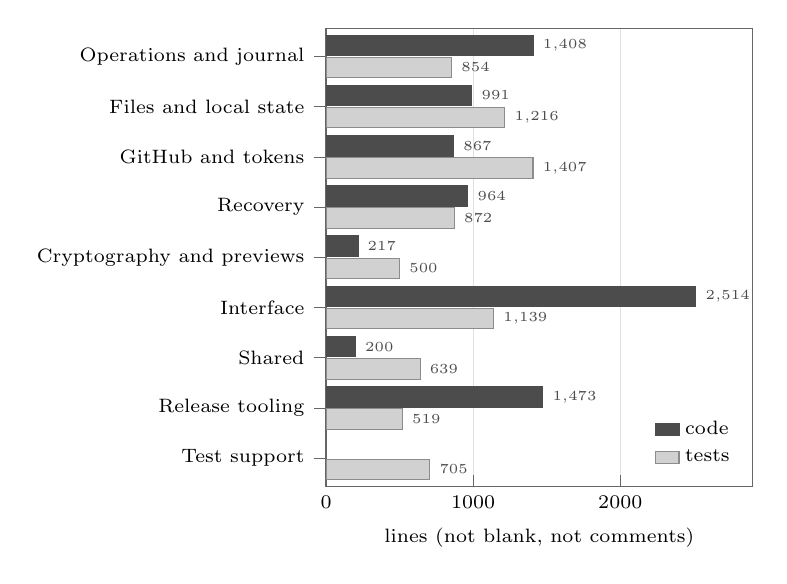
\begin{tikzpicture}
\begin{axis}[
  xbar=0.6pt, width=70mm, height=74mm,
  font=\scriptsize,
  bar width=2.6mm,
  xmin=0, xmax=2900, xtick={0,1000,2000}, xticklabels={0,1000,2000},
  scaled x ticks=false,
  xlabel={lines (not blank, not comments)},
  y dir=reverse, ytick=data, enlarge y limits=0.07,
  symbolic y coords={Operations and journal, Files and local state, GitHub and tokens, Recovery,
                     Cryptography and previews, Interface, Shared, Release tooling, Test support},
  yticklabel style={align=right},
  axis line style={black!60}, tick style={black!60},
  xmajorgrids, grid style={black!12},
  legend style={font=\scriptsize, draw=none, at={(0.98,0.02)}, anchor=south east, cells={anchor=west}},
  reverse legend,
  legend image code/.code={\draw[#1] (0mm,-0.8mm) rectangle (3mm,0.8mm);},
  xtick pos=bottom, ytick pos=left,
  nodes near coords, nodes near coords style={font=\tiny, text=black!70},
  every node near coord/.append style={anchor=west},
]
\addplot[fill=black!18, draw=black!45] coordinates {
  (854,Operations and journal) (1216,Files and local state) (1407,GitHub and tokens) (872,Recovery)
  (500,Cryptography and previews) (1139,Interface) (639,Shared) (519,Release tooling) (705,Test support)};
\addlegendentry{tests}
\addplot[fill=black!70, draw=black!70] coordinates {
  (1408,Operations and journal) (991,Files and local state) (867,GitHub and tokens) (964,Recovery)
  (217,Cryptography and previews) (2514,Interface) (200,Shared) (1473,Release tooling)};
\addlegendentry{code}
\end{axis}
\end{tikzpicture}

\caption{Lines of code per component, and of the tests assigned to the component they mainly
exercise. Counted by \code{report/data/code\_size.py}: lines that are neither blank nor comments;
docstrings count.}
\label{fig:size}
\end{figure}

\section{Verification}\label{sec:verification}

\subsection{The test suite}
The automated suite has 663 tests in 20 modules (\tabref{tab:tests}). Except for the optional
real-GitHub tests, they run the real \code{Vault} against a simulated GitHub: an in-memory model of
the endpoints GhostVault uses that keeps what decides correctness, namely content-addressed blobs with
real Git ids, immutable trees and commits, branch updates that must fast-forward, recursive listings
and their truncation, empty repositories that answer 409 until initialised, private, archived and
read-only repositories, and tokens that stop working. A deletion is a new commit, so deleted blobs
stay in the history, as on GitHub. Nothing touches the network.

\begin{table*}[t]
\caption{The test modules}\label{tab:tests}
\centering\footnotesize
\setlength{\tabcolsep}{4pt}
\begin{tabularx}{\textwidth}{@{}L{25mm}rY@{\hspace{10pt}}L{25mm}rY@{}}
\toprule
\textbf{Module} & \textbf{Tests} & \textbf{What it checks} & \textbf{Module} & \textbf{Tests} & \textbf{What it checks} \\
\midrule
\code{resilience} & 90 & retries, backoff, rate limits, pacing, uncertain outcomes, transport, fault schedules & \code{credentials} & 30 & keychain selection, session fallback, accepted repositories \\ \addlinespace[1.6pt]
\code{gui} & 58 & the real Tk window: background work, layout, scaling, keyboard, secrets & \code{placement} & 24 & distributed and consolidated placement \\ \addlinespace[1.6pt]
\code{security} & 53 & tampered and damaged records, what decryption binds, malicious input, leaks & \code{local\_state} & 23 & the data folder, permissions, damage, the lock \\ \addlinespace[1.6pt]
\code{original\_file} & 51 & which files are accepted; reading safely; the deletion race & \code{gallery} & 17 & encrypted previews and renaming \\ \addlinespace[1.6pt]
\code{recovery} & 49 & recovery files and the repository backup, end to end & \code{restore\_safety} & 16 & never replacing a file; flushing before remote deletion \\ \addlinespace[1.6pt]
\code{packaging} & 43 & the build script, the PyInstaller specification, the install scripts & \code{compatibility} & 16 & records of format 5, written by an earlier version's own code \\ \addlinespace[1.6pt]
\code{journal} & 41 & an interruption at each checkpoint, then start-up recovery & \code{real\_github} & 14 & optional: the same operations on real repositories \\ \addlinespace[1.6pt]
\code{units} & 41 & helpers, atomic writes, start-up, self-check, TLS & \code{remote\_cleanup} & 13 & removal that GitHub refuses or applies only in part \\ \addlinespace[1.6pt]
\code{ghost\_and\_restore} & 38 & the core cycle and its failure modes & \code{github\_layer} & 10 & what the GitHub layer verifies; streaming without staging \\ \addlinespace[1.6pt]
\code{backup\_integrity} & 31 & incomplete records never shrink a backup & \code{logging} & 5 & the log never holds an exception's message \\
\bottomrule
\end{tabularx}
\end{table*}

Four techniques carry most of the weight.
\emph{Simulated crashes:} a test harness stops the vault at a named checkpoint by raising an exception
that none of GhostVault's error handling catches, as when a process dies; it then starts a new vault on
the same folder, runs start-up recovery, and checks that the file is in at least one place byte for
byte (the original, a restorable ghost, or the restored file), that every chunk on GitHub is accounted
for by a record, and that no temporary file is left. Every checkpoint in the code is covered.
\emph{Faults:} requests fail before GitHub acts or after it acted with the reply lost, on schedules that
are a pure function of a seed and the request itself, so parallel downloads cannot change which
requests fail and every run is exactly reproducible.
\emph{Property tests:} seeded random damage to recovery files (300 cases) and records (250 cases)
must be refused or fail closed, never give wrong bytes; padding is checked at 40 random sizes.
\emph{The real interface:} the GUI tests drive the Tk window itself (under Xvfb on Linux) and are
written to hold on Tk 8.6 and Tk 9 and at any display scale.

The suite checks outcomes, not the absence of exceptions: the bytes restored, the original still
present, what is on the simulated GitHub, file modes, and what the user is told. The real-GitHub tests
run only with dedicated repositories and a token supplied in the environment.

\subsection{Crashes and faults together}\label{sec:stress}
A separate tool, \code{tools/stress.py}, runs long random sequences of operations against the
simulated GitHub with two repositories and a 4\,KiB chunk size, so that files have many chunks. Each
cycle ghosts a new random file (of a size chosen among the edge cases 0, 1, 4\,095, 4\,096 and
4\,097 bytes and random sizes up to twelve chunks, with random placement and padding) or restores a
random ghost. With a given probability the operation is stopped at a random checkpoint and GhostVault
is restarted on the same folder; network faults are injected throughout, transient as on a real
network (no request fails more than three times in a row). After every cycle the invariants of the
crash tests are checked; at the end every ghost is restored, start-up recovery runs once more, and
GitHub must hold no chunk at all.

Eight runs were made: five with a crash probability of 0.35 and a fault rate of 0.05, and three with
0.5 and 0.15, 400 cycles each. Together they executed 3\,200 operations, stopped 1\,273 of them at a
checkpoint (\figref{fig:crashes}), injected 7\,736 network faults, ran start-up recovery 1\,273 times
and checked the invariants 3\,208 times. Every invariant held in every run: no file was lost, no chunk
was left unaccounted for, every ghost restored byte for byte, and GitHub was empty at the end. The runs
took 61\,s in total. This test stops the process at checkpoints; the file system itself stays
consistent, so it does not simulate a power failure, which the ordering of flushes
(\secref{sec:durable}) is designed for but which was not tested.

\begin{figure}[t]
\centering
% Fig.: simulated crashes per checkpoint in the stress runs (report/data/stress.json), in the
% order the checkpoints are reached.
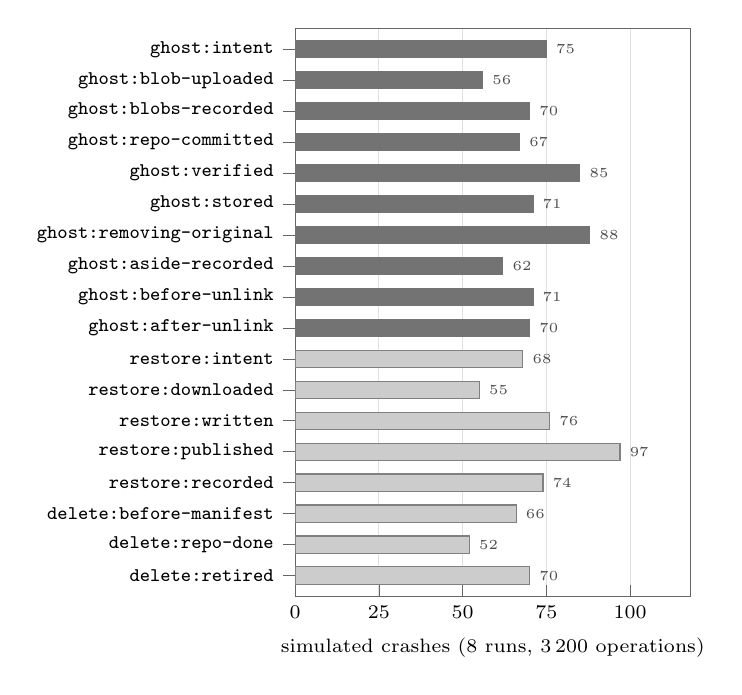
\begin{tikzpicture}
\begin{axis}[
  xbar, bar shift=0pt, width=66mm, height=88mm,
  font=\scriptsize,
  bar width=2.2mm,
  xmin=0, xmax=118, xtick={0,25,50,75,100},
  xlabel={simulated crashes (8 runs, 3\,200 operations)},
  y dir=reverse, enlarge y limits=0.04,
  ytick={ghost:intent, ghost:blob-uploaded, ghost:blobs-recorded, ghost:repo-committed,
                     ghost:verified, ghost:stored, ghost:removing-original, ghost:aside-recorded,
                     ghost:before-unlink, ghost:after-unlink, restore:intent, restore:downloaded,
                     restore:written, restore:published, restore:recorded, delete:before-manifest,
                     delete:repo-done, delete:retired},
  xtick pos=bottom, ytick pos=left,
  symbolic y coords={ghost:intent, ghost:blob-uploaded, ghost:blobs-recorded, ghost:repo-committed,
                     ghost:verified, ghost:stored, ghost:removing-original, ghost:aside-recorded,
                     ghost:before-unlink, ghost:after-unlink, restore:intent, restore:downloaded,
                     restore:written, restore:published, restore:recorded, delete:before-manifest,
                     delete:repo-done, delete:retired},
  yticklabel style={font=\scriptsize\ttfamily},
  axis line style={black!60}, tick style={black!60},
  xmajorgrids, grid style={black!12},
  nodes near coords, nodes near coords style={font=\tiny, text=black!70, anchor=west},
]
\addplot[fill=black!55, draw=black!55] coordinates {
  (75,ghost:intent) (56,ghost:blob-uploaded) (70,ghost:blobs-recorded) (67,ghost:repo-committed)
  (85,ghost:verified) (71,ghost:stored) (88,ghost:removing-original) (62,ghost:aside-recorded)
  (71,ghost:before-unlink) (70,ghost:after-unlink)};
\addplot[fill=black!20, draw=black!50] coordinates {
  (68,restore:intent) (55,restore:downloaded) (76,restore:written) (97,restore:published)
  (74,restore:recorded) (66,delete:before-manifest) (52,delete:repo-done) (70,delete:retired)};
\end{axis}
\end{tikzpicture}

\caption{Where the stress runs stopped the process: the 18 checkpoints of ghosting (dark) and of
restoring and removing (light), in the order they are reached. Data: \code{report/data/stress.json}.}
\label{fig:crashes}
\end{figure}

\subsection{What was verified, and where}\label{sec:status}
\tabref{tab:status} lists what was run for the version this report describes, on what, and with what
result. All of it ran on one Linux x86-64 machine. Windows and macOS were not available there,
GitHub Actions was not run, PyInstaller could not be installed for lack of access to the package
index, and no real GitHub repository was used.

\begin{table*}[t]
\caption{Verification status of GhostVault 1.0.0}\label{tab:status}
\centering\footnotesize
\begin{tabularx}{\textwidth}{@{}L{60mm}L{50mm}Y@{}}
\toprule
\textbf{What} & \textbf{Where} & \textbf{Result} \\
\midrule
The test suite, Python 3.13.14 with Tk 9.0.3, under Xvfb & Linux x86-64 (Ubuntu 24.04), as root &
640 passed, 23 skipped: 14 need real GitHub, 6 Windows, 2 a non-root user, 1 the machine's keychain \\ \addlinespace[1.6pt]
The test suite, Python 3.11 and 3.14 with Tk 9.0 & the same & 638 passed, 2 failed, 23 skipped each; both failures from this machine's builds of the dependencies (below) \\ \addlinespace[1.6pt]
The test suite, Python 3.12 with Tk 8.6.15 & the same & the same as for 3.11 and 3.14 \\ \addlinespace[1.6pt]
The test suite as an unprivileged user, Python 3.13 & the same & not completed (run stopped) \\ \addlinespace[1.6pt]
The core without Tk (system Python 3.13, no \code{tkinter}) & the same & 575 passed, 86 skipped (GUI), 2 failed as above \\ \addlinespace[1.6pt]
Lint: \code{ruff}; \code{shellcheck} on the install scripts; \code{actionlint} (with
\code{shellcheck}) on the three workflows & the same & no findings \\ \addlinespace[1.6pt]
The wheel: built, contents checked, installed into an empty environment and started & the same &
not run for this version \\ \addlinespace[1.6pt]
The PyInstaller specification: executed with stand-ins for PyInstaller under Linux, Windows and
macOS settings; type-checked against PyInstaller's type stubs & the same & spec tests passed; type check not run for this version \\ \addlinespace[1.6pt]
\code{build.py} after freezing (smoke test, packaging, verification with install, update and
uninstall), on a stand-in for PyInstaller's output folder & the same & not run for this version \\ \addlinespace[1.6pt]
The stress runs (\secref{sec:stress}) and the measurements (\secref{sec:performance}) & the same,
Python 3.13 & every invariant held; measurements as reported \\
\midrule
\multicolumn{3}{@{}p{\textwidth}@{}}{\emph{The two failures outside Python 3.13 are environmental: the Pillow built here for
those interpreters has no JPEG encoder, which \code{--self-check} rightly reports as missing; and the
\code{packaging} distribution was absent, so a test imported the project's own \code{packaging/} folder
instead (the test now skips in that case).}} \\ \addlinespace[1.6pt]
\midrule
The test suite on Windows and macOS (the CI matrix) & --- & not run \\ \addlinespace[1.6pt]
The real-GitHub tests & --- & not run \\ \addlinespace[1.6pt]
PyInstaller itself, the standalone applications, the Windows installer, the disk images, code
signing, notarization, and the release workflow & --- & not run \\
\bottomrule
\end{tabularx}
\end{table*}

\section{Performance}\label{sec:performance}

\subsection{Method}
\code{tools/measure.py} measures GhostVault's own costs against the simulated GitHub, which runs in
the same process; the results are in \code{report/data/measurements.json}. Times are therefore
GhostVault's work plus the simulator's, plus an optional delay added to every request; they are not
GitHub's. What GitHub adds is reported separately, as counts of requests. Write pacing, which on
GitHub spaces writes at least one second apart, is turned off for the timing, and its cost is given
instead as a lower bound: one second per write request. Each measurement runs twice, once for time and
requests and once, traced, for peak memory, because tracing slows Python down. Peak memory is what
Python allocates during the operation, minus the simulated GitHub's copy of the blobs. The machine was a
virtual machine with two cores of an Intel Xeon at 2.10\,GHz, Linux 6.18, Python 3.13.14 and
\code{cryptography} 50.0.1 with OpenSSL 4.0.2, using two repositories and the default distributed placement. The measurements and the stress runs were made on the code as it was just before the final validation check of \secref{sec:records} was added, one check per record read.

\subsection{Primitives}
Working on one 512\,KiB chunk at a time, AES-256-GCM encrypted at 1\,603\,MiB/s and decrypted at
1\,755\,MiB/s; SHA-256
ran at 1\,313\,MiB/s and the Git blob id at 1\,403\,MiB/s. Deriving a recovery bundle's key with the
default Argon2id parameters took 0.64\,s at best and 0.68\,s at the median of five runs. The
cryptography is far from being what limits GhostVault.

\subsection{Ghosting and restoring}
\tabref{tab:cycles} and \figref{fig:perf} show complete cycles of random (incompressible, non-image)
files of 1 to 256\,MiB. The requests a ghost makes follow from the design: one blob per chunk, then for
each repository one tree, one commit and one branch update, plus the reads that check the repository
and verify the upload; the first ghost in an empty repository also initialises it. A ghost of $n$
chunks over two repositories thus made $n+8$ writes here, $n+6$ in repositories already initialised.
A restore downloads each chunk once, reads the branches a few times, and makes six writes, the
deletion commits. Peak memory stayed between
3.5 and 6.5\,MiB whatever the file size, because chunks are streamed, and the data folder never held
more than the record: nothing is staged on disk.

\begin{table}[t]
\caption{Ghost and restore cycles (no added delay)}\label{tab:cycles}
\centering\footnotesize
\setlength{\tabcolsep}{4.2pt}
\begin{tabular}{@{}rrrrrrr@{}}
\toprule
& & \multicolumn{3}{c}{\textbf{Ghost}} & \multicolumn{2}{c}{\textbf{Restore}} \\
\cmidrule(lr){3-5}\cmidrule(l){6-7}
\textbf{MiB} & \textbf{Chunks} & \textbf{Time} & \textbf{Req.} & \textbf{Writes} & \textbf{Time} &
\textbf{Req.} \\
\midrule
1 & 2 & 0.037\,s & 24 & 10 & 0.041\,s & 22 \\
16 & 32 & 0.203\,s & 56 & 40 & 0.335\,s & 52 \\
64 & 128 & 0.875\,s & 152 & 136 & 1.263\,s & 148 \\
256 & 512 & 4.189\,s & 536 & 520 & 4.585\,s & 532 \\
\bottomrule
\end{tabular}

\vspace{2pt}\raggedright\scriptsize Two repositories, each initialised by the ghost. A restore always
made 6 writes. With 20\,ms added to every request: 1\,MiB, ghost 0.533\,s, restore 0.471\,s;
16\,MiB, ghost 1.406\,s, restore 0.730\,s.
\end{table}

\begin{figure}[t]
\centering
% Fig.: time of a ghost and of a restore against the simulated GitHub (report/data/measurements.json),
% and the lower bound GitHub's write pacing puts on the same operations.
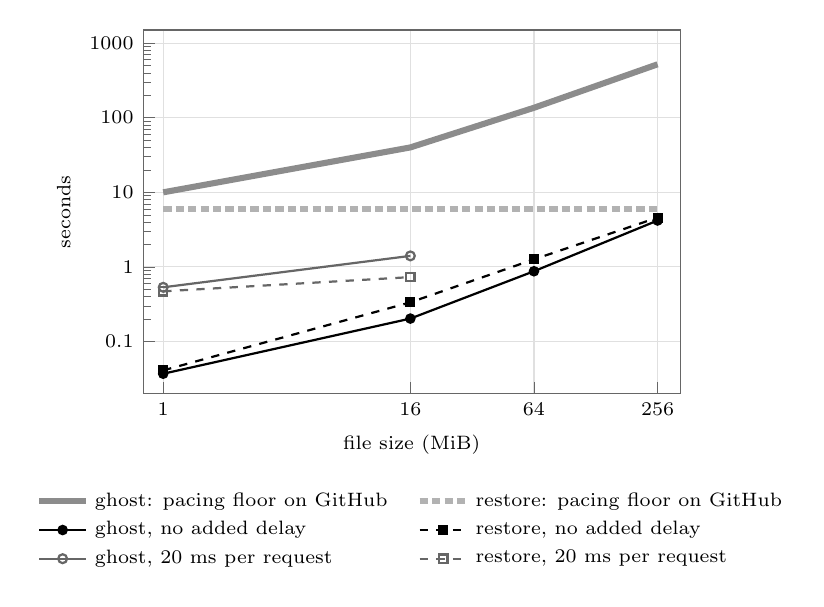
\begin{tikzpicture}
\begin{loglogaxis}[
  width=84mm, height=62mm,
  font=\scriptsize,
  xlabel={file size (MiB)}, ylabel={seconds},
  xmin=0.8, xmax=330, ymin=0.02, ymax=1500,
  xtick={1,16,64,256}, xticklabels={1,16,64,256},
  ytick={0.1,1,10,100,1000}, yticklabels={0.1,1,10,100,1000},
  grid=major, grid style={black!12},
  axis line style={black!60}, tick style={black!60},
  xtick pos=bottom, ytick pos=left,
  legend columns=2,
  legend style={font=\scriptsize, draw=none, at={(0.5,-0.24)}, anchor=north, cells={anchor=west},
                /tikz/every even column/.append style={column sep=3mm}},
  legend cell align=left,
  every axis plot/.append style={every mark/.append style={solid}},
]
\addplot[black!45, line width=2.2pt, mark=none] coordinates {(1,10) (16,40) (64,136) (256,520)};
\addlegendentry{ghost: pacing floor on GitHub}
\addplot[black!30, line width=2.2pt, mark=none, dash pattern=on 3pt off 1.5pt] coordinates {(1,6) (16,6) (64,6) (256,6)};
\addlegendentry{restore: pacing floor on GitHub}
\addplot[black, thick, mark=*, mark size=1.5pt] coordinates {(1,0.037) (16,0.203) (64,0.875) (256,4.189)};
\addlegendentry{ghost, no added delay}
\addplot[black, thick, mark=square*, mark size=1.4pt, dashed] coordinates {(1,0.041) (16,0.335) (64,1.263) (256,4.585)};
\addlegendentry{restore, no added delay}
\addplot[black!60, thick, mark=o, mark size=1.6pt] coordinates {(1,0.533) (16,1.406)};
\addlegendentry{ghost, 20 ms per request}
\addplot[black!60, thick, mark=square, mark size=1.5pt, dashed] coordinates {(1,0.471) (16,0.730)};
\addlegendentry{restore, 20 ms per request}
\end{loglogaxis}
\end{tikzpicture}

\caption{Time of a ghost and of a restore against the simulated GitHub, and the lower bound that
GitHub's write pacing (one write per second) puts on the same operations on GitHub. Both axes are
logarithmic. The 20\,ms series show the effect of request latency: a ghost's requests are sequential,
while a restore downloads eight chunks at a time.}
\label{fig:perf}
\end{figure}

\subsection{What GitHub adds}
On GitHub the floor dominates. At one write per second, a ghost of 256\,MiB needs at least 520\,s,
whatever the network: GhostVault can upload at most 512\,KiB per second, about 1.76\,GiB per hour,
before transfer time is even counted, and each chunk travels as base64 inside JSON, a third larger
than its ciphertext. GitHub also limits content creation to 80 requests per minute and 500 per
hour~\cite{gh-rate}, without listing which endpoints count. If blob creation counts against the hourly
limit, an account can store at most about 250\,MiB of chunks per hour, and GhostVault waits whenever
GitHub signals the limit. None of these costs was measured on GitHub. A restore is bound instead by
download bandwidth and by the primary limit of 5\,000 requests per hour per token~\cite{gh-rate},
which corresponds to about 2.4\,GiB of chunks per hour. Removing a ghost costs a few writes per
repository, whatever its size.

\subsection{Many ghosts}
\tabref{tab:scaling} shows the costs that grow with the number of ghosts. Each record takes about
1.6\,KB. Listing and start-up recovery read and validate every record, which is linear and cheap. Making
a ghost, however, also reads every record, to check that its name is unique, so the cost per ghost
grows linearly with their number, from 0.026\,s with 100 ghosts to 0.124\,s with 3\,000; on GitHub,
where even a one-chunk ghost takes a few seconds of paced writes, this is still small.

\begin{table}[t]
\caption{Costs that grow with the number of ghosts}\label{tab:scaling}
\centering\footnotesize
\begin{tabular}{@{}rrrr@{}}
\toprule
\textbf{Ghosts} & \textbf{Ghost one more} & \textbf{List all} & \textbf{Start-up recovery} \\
\midrule
100 & 0.026\,s & 0.005\,s & 0.011\,s \\
1\,000 & 0.056\,s & 0.070\,s & 0.164\,s \\
3\,000 & 0.124\,s & 0.170\,s & 0.644\,s \\
\bottomrule
\end{tabular}

\vspace{2pt}\raggedright\scriptsize Ghosts of 100 bytes, one chunk each, without previews; ``ghost one
more'' is the average over all ghosts made.
\end{table}

\section{Limitations}\label{sec:limitations}

\emph{A ghost is a single copy.} Every chunk is stored once, in one repository, and GhostVault never
makes a second copy. Placement spreads storage; it does not protect against losing a repository, and
distributed placement makes a file depend on every repository that holds one of its chunks. What
GitHub deletes, loses or withholds cannot be brought back, and the user's use of GitHub is subject to
GitHub's terms, including its limits on repository size, request rates and bandwidth. Files that
cannot be lost need another copy elsewhere.

\emph{Removed is not erased.} Restoring a ghost removes its chunks from the branch, not from Git's
history, and GitHub may keep unreachable objects for a time. Every earlier version of the repository
backup stays in history too. A removed file stays unreadable only while its key exists nowhere. Getting
rid of old objects for good requires deleting the repository, or rewriting its history and asking
GitHub to purge cached objects. On SSDs and copy-on-write file systems, deleting the original does not
reliably destroy its old content either.

\emph{Keys at rest and in memory.} File keys are stored unencrypted in owner-only files
(\secref{sec:keys}), so anyone who can read the data folder, or a backup of it, and the repositories
can decrypt the files. Keys, passphrases and tokens pass through process memory, which Python cannot
reliably erase; swap, hibernation files and crash dumps may hold them.

\emph{The deletion window on Linux and macOS.} A program that already had the original open for
writing can still write to it in the moment between GhostVault's last check and the deletion
(\secref{sec:remove}). Windows closes that window; Linux and macOS offer no way to.

\emph{Metadata.} GitHub learns what \tabref{tab:learn} lists: how much is stored, approximate sizes,
and when ghosts come and go. A preview's existence reveals that a ghost is probably an image.

\emph{Throughput.} GitHub's pacing and limits, not GhostVault, bound how fast files can be ghosted
(\secref{sec:performance}); a large file takes minutes to hours, and GhostVault waits whenever GitHub
asks it to. Making a ghost also costs time linear in the number of ghosts.

\emph{One computer at a time.} A data folder is used by one GhostVault process at a time. Two
computers can share repositories, and the backup detects ghosts it does not know, but they do not
share or merge ghosts.

\emph{Scope.} Only repositories on \code{github.com} are supported, one file is ghosted at a time,
and folders are not. Tk exposes little to screen readers; every action can be reached from the
keyboard, but GhostVault cannot do more without leaving Tk. Standalone builds are unsigned unless a
signing certificate is configured, and there is no automatic update.

\emph{Verification.} The limits of what was verified are listed in \secref{sec:status}: the Windows
and macOS behaviour, the real-GitHub tests, the release workflow and the standalone applications were
not run for the version described here.

\section{Conclusion}\label{sec:conclusion}

GhostVault keeps files in private GitHub repositories without trusting GitHub with them. The
cryptography is conventional: a random key per file, AES-256-GCM per chunk, associated data that binds
each chunk to its file, position, count, size and padding, and keys for recovery bundles derived with
Argon2id. Most of the system is about something else: deleting the user's data only when another copy
has been shown to exist. The original goes only after the branch has been read back and a sample
downloaded, and after the file has been moved aside and checked again; the remote copy goes only after
the restored file is on disk under its final name. Every step that changes something outside the
computer is journaled first, every reply that matters is checked against what the repository shows,
and every record is validated before anything acts on it.

The protection has clear edges. Cryptography protects the content of files from everyone who can read
the repositories; GitHub's access control decides who those readers are; and only GitHub keeps the data
available, which is why a ghost should never be the only copy of a file that cannot be lost. Within
those edges, the system was checked by an automated suite covering every journal checkpoint, by
randomised runs in which 1\,273 simulated crashes and 7\,736 network faults lost no file, and by
measurements showing that the limit on its speed is GitHub's pacing, not its own work.

\section*{Availability}
GhostVault is open source under the MIT license. The source, its documentation, the test suite, the
measurement and stress tools, and this report's \LaTeX{} source and data are in the project's
repository.

\begingroup
\footnotesize
\setlength{\itemsep}{1pt}
\renewcommand{\refname}{References}
\begin{thebibliography}{99}
\setlength{\itemsep}{1.5pt}

\bibitem{gh-large} GitHub, ``About large files on GitHub,'' GitHub Docs. [Online]. Available:
\url{https://docs.github.com/en/repositories/working-with-files/managing-large-files/about-large-files-on-github}
(accessed Oct.\ 2026).

\bibitem{gh-aup} GitHub, ``GitHub Acceptable Use Policies,'' GitHub Docs, Sec.~9, ``Excessive
Bandwidth Use.'' [Online]. Available:
\url{https://docs.github.com/en/site-policy/acceptable-use-policies/github-acceptable-use-policies}
(accessed Oct.\ 2026).

\bibitem{nist-gcm} M. Dworkin, ``Recommendation for block cipher modes of operation: Galois/Counter
Mode (GCM) and GMAC,'' NIST Special Publication 800-38D, Nov.\ 2007.

\bibitem{rfc5869} H. Krawczyk and P. Eronen, ``HMAC-based extract-and-expand key derivation function
(HKDF),'' RFC 5869, May 2010.

\bibitem{rfc9106} A. Biryukov, D. Dinu, D. Khovratovich, and S. Josefsson, ``Argon2 memory-hard
function for password hashing and proof-of-work applications,'' RFC 9106, Sept.\ 2021.

\bibitem{rfc7914} C. Percival and S. Josefsson, ``The scrypt password-based key derivation
function,'' RFC 7914, Aug.\ 2016.

\bibitem{rfc2104} H. Krawczyk, M. Bellare, and R. Canetti, ``HMAC: Keyed-hashing for message
authentication,'' RFC 2104, Feb.\ 1997.

\bibitem{pyca} Python Cryptographic Authority, ``cryptography.'' [Online]. Available:
\url{https://cryptography.io/}

\bibitem{git-objects} S. Chacon and B. Straub, \emph{Pro Git}, 2nd ed. Apress, 2014, Sec.~10.2,
``Git objects.''

\bibitem{gh-git} GitHub, ``REST API endpoints for Git trees'' and the other Git database endpoints
(blobs, commits, references), GitHub Docs. [Online]. Available: \url{https://docs.github.com/en/rest/git}
(accessed Oct.\ 2026).

\bibitem{truststore} S. M. Larson et al., ``truststore: verify certificates using native system trust
stores.'' [Online]. Available: \url{https://github.com/sethmlarson/truststore}

\bibitem{gh-best} GitHub, ``Best practices for using the REST API,'' GitHub Docs. [Online]. Available:
\url{https://docs.github.com/en/rest/using-the-rest-api/best-practices-for-using-the-rest-api}
(accessed Oct.\ 2026).

\bibitem{gh-rate} GitHub, ``Rate limits for the REST API,'' GitHub Docs. [Online]. Available:
\url{https://docs.github.com/en/rest/using-the-rest-api/rate-limits-for-the-rest-api}
(accessed Oct.\ 2026).

\bibitem{crockford} D. Crockford, ``Base 32.'' [Online]. Available:
\url{https://www.crockford.com/base32.html}

\bibitem{pyinstaller} PyInstaller Development Team, ``PyInstaller.'' [Online]. Available:
\url{https://pyinstaller.org/}

\bibitem{keyring} J. R. Coombs et al., ``keyring.'' [Online]. Available:
\url{https://github.com/jaraco/keyring}

\end{thebibliography}
\endgroup


\end{document}
